\documentclass[paper=a4,fontsize=11pt]{article}
\usepackage[left=2.5cm,right=2.5cm,top=2.5cm,bottom=2.5cm]{geometry}
\usepackage[english]{babel} 
\usepackage[]{graphicx}
\usepackage{floatrow}
\usepackage{subfig}
\floatsetup[figure]{style=plain,subcapbesideposition=top}


\begin{document}


\vspace*{\fill}
\noindent\makebox[\textwidth]{\Huge Appendix}
\vfill
\thispagestyle{empty}
\newpage


\section{Unmitigated Strategy}
\newpage


\subsection{Swine Flu}

\begin{figure}[!h]
  \sidesubfloat[]{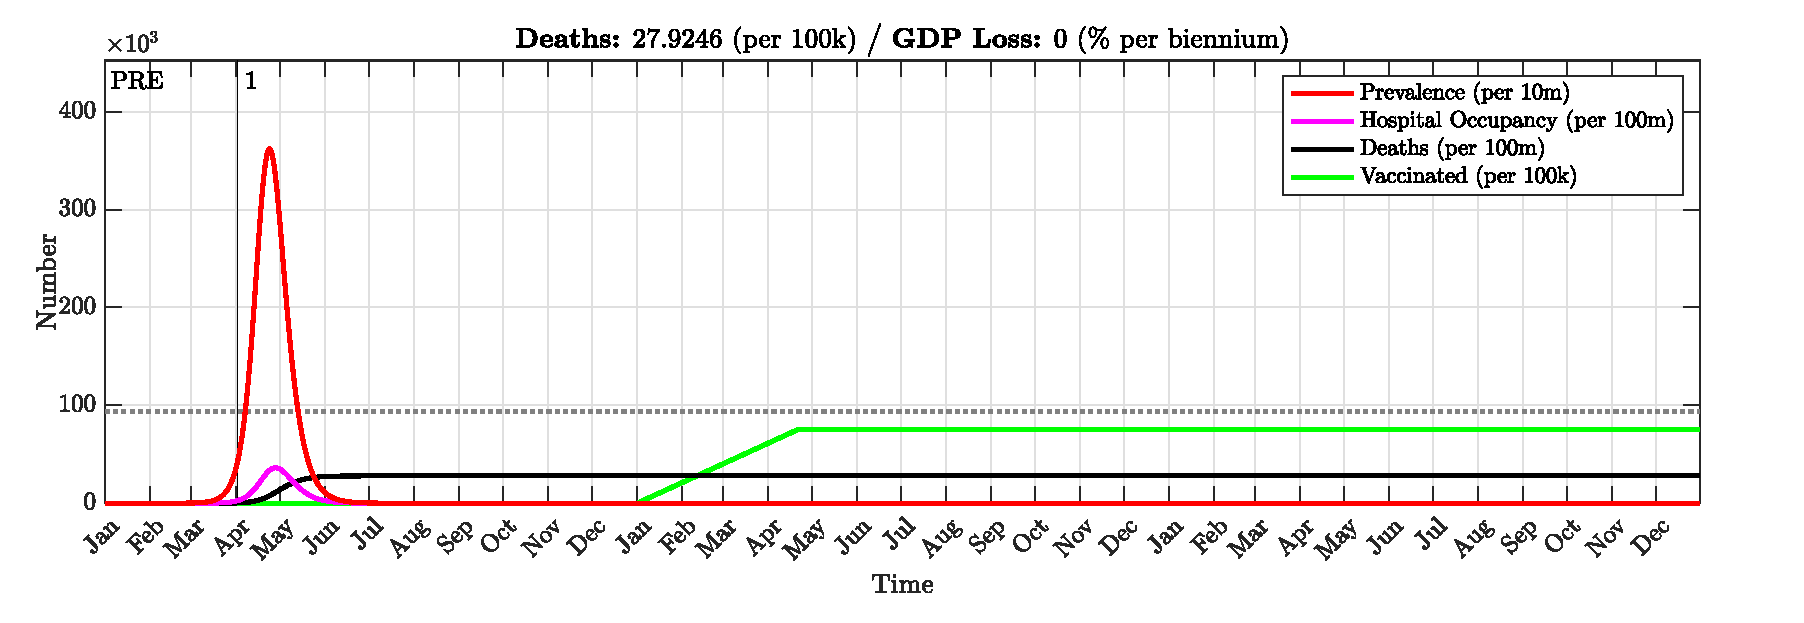
\includegraphics[width=0.95\textwidth,height=5cm]{Unmitigated/Counterfactuals/US_swfl}}\\
  \sidesubfloat[]{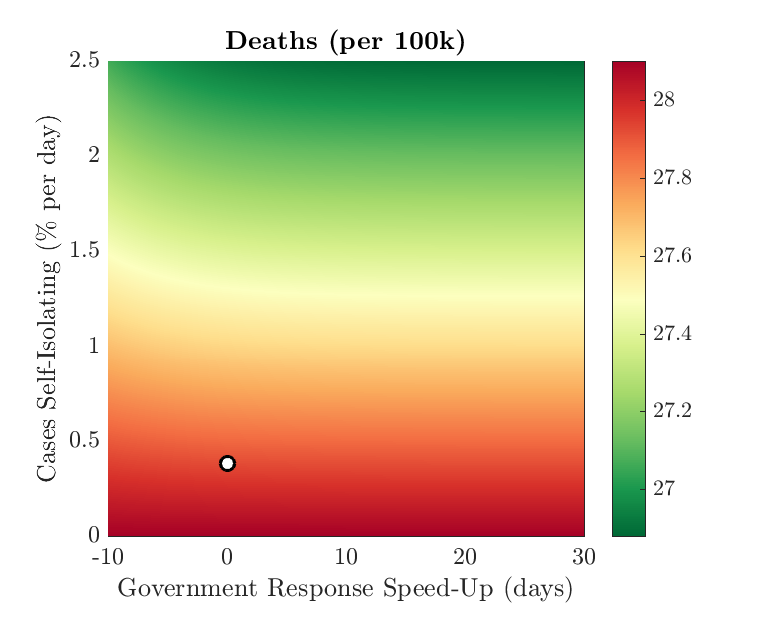
\includegraphics[width=0.40\textwidth,height=5cm]{Unmitigated/US/SWINE/ero_d}}\hspace{1.8cm}
  \sidesubfloat[]{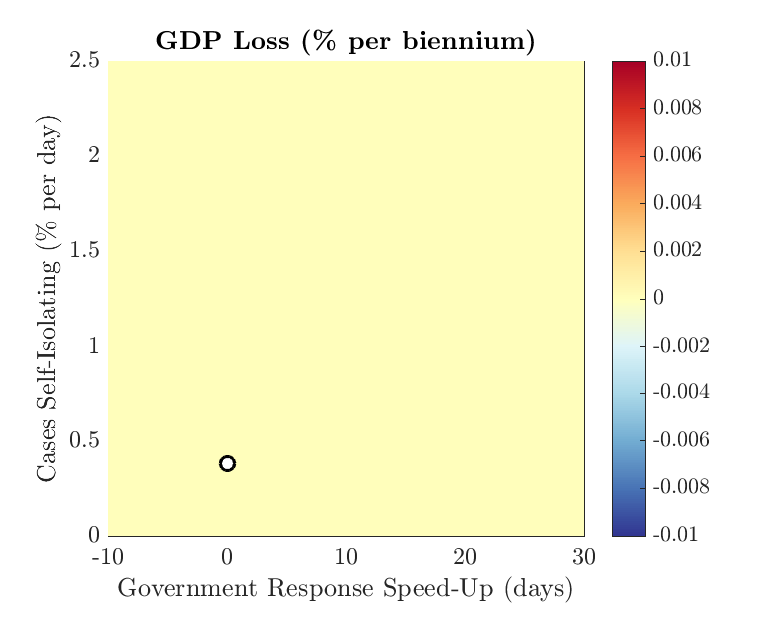
\includegraphics[width=0.40\textwidth,height=5cm]{Unmitigated/US/SWINE/ero_g}}\\
  \sidesubfloat[]{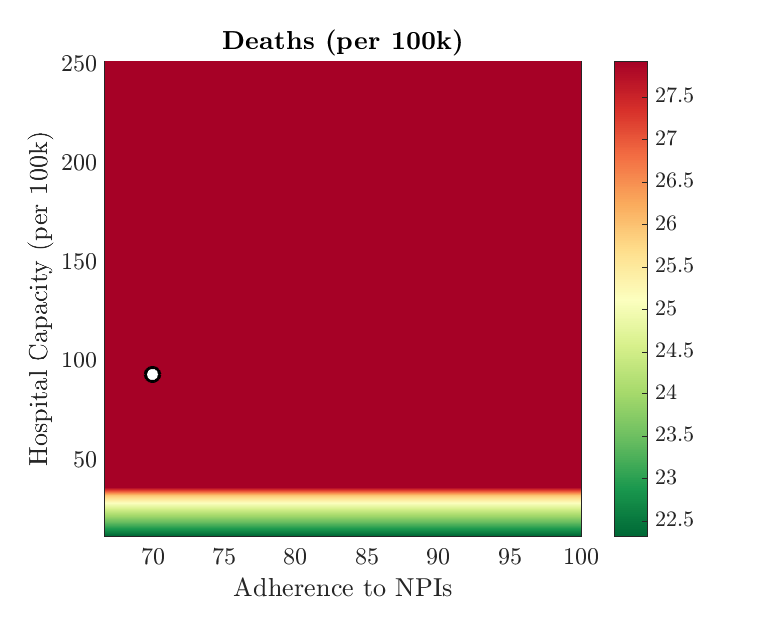
\includegraphics[width=0.40\textwidth,height=5cm]{Unmitigated/US/SWINE/npl_d}}\hspace{1.8cm}
  \sidesubfloat[]{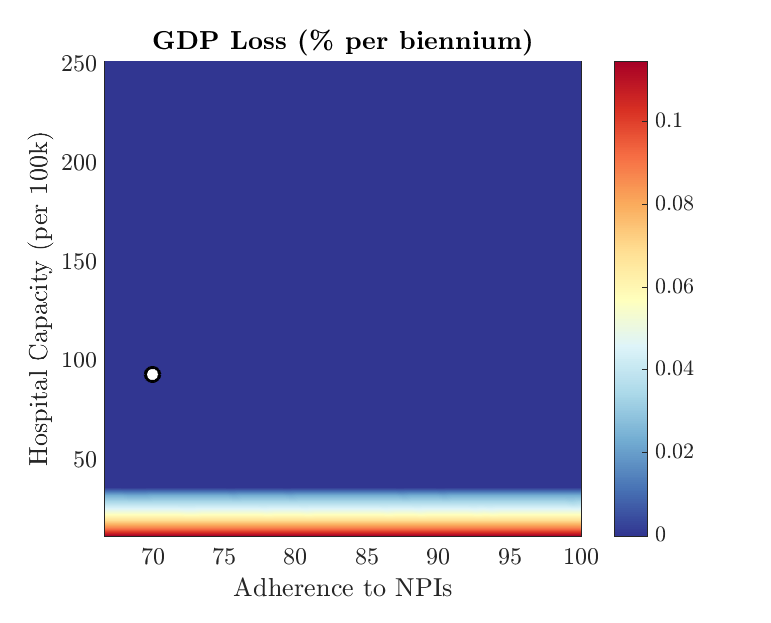
\includegraphics[width=0.40\textwidth,height=5cm]{Unmitigated/US/SWINE/npl_g}}\\
  \sidesubfloat[]{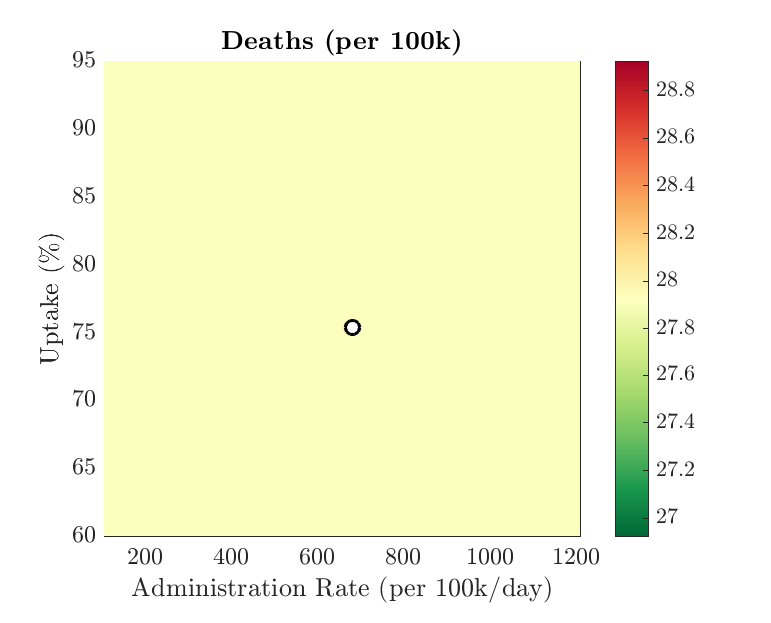
\includegraphics[width=0.40\textwidth,height=5cm]{Unmitigated/US/SWINE/imm_d}}\hspace{1.76cm}
  \sidesubfloat[]{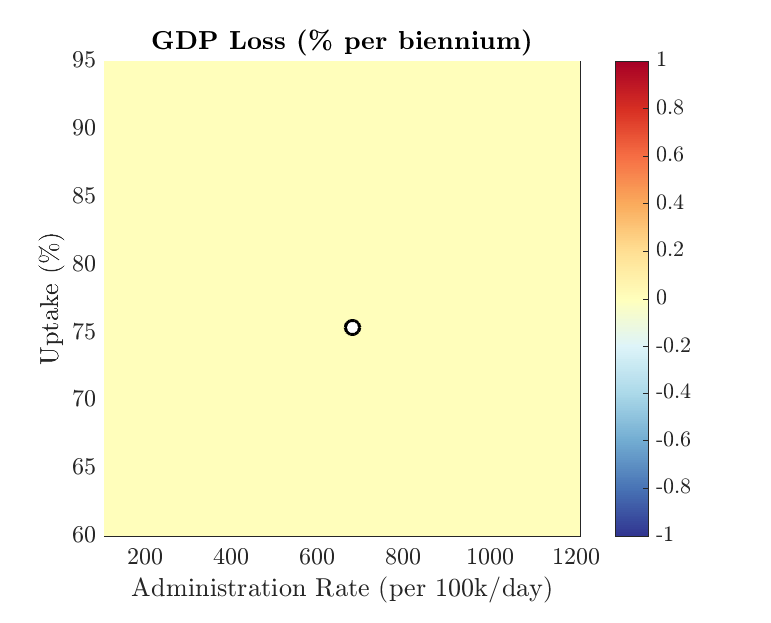
\includegraphics[width=0.40\textwidth,height=5cm]{Unmitigated/US/SWINE/imm_g}}\\
  \caption*{\textbf{Figure A1:} P2 in the USA; $(a)$ the counterfactual epidemic trajectory; the effects of increasing/decreasing $(b,c)$ the government response time \& proportion of cases self-isolating, $(d,e)$ adherence to NPIs during lockdown \& hospital capacity, and $(f,g)$ vaccine administration rate \& uptake.}
\end{figure}

\begin{figure}[!h]
  \sidesubfloat[]{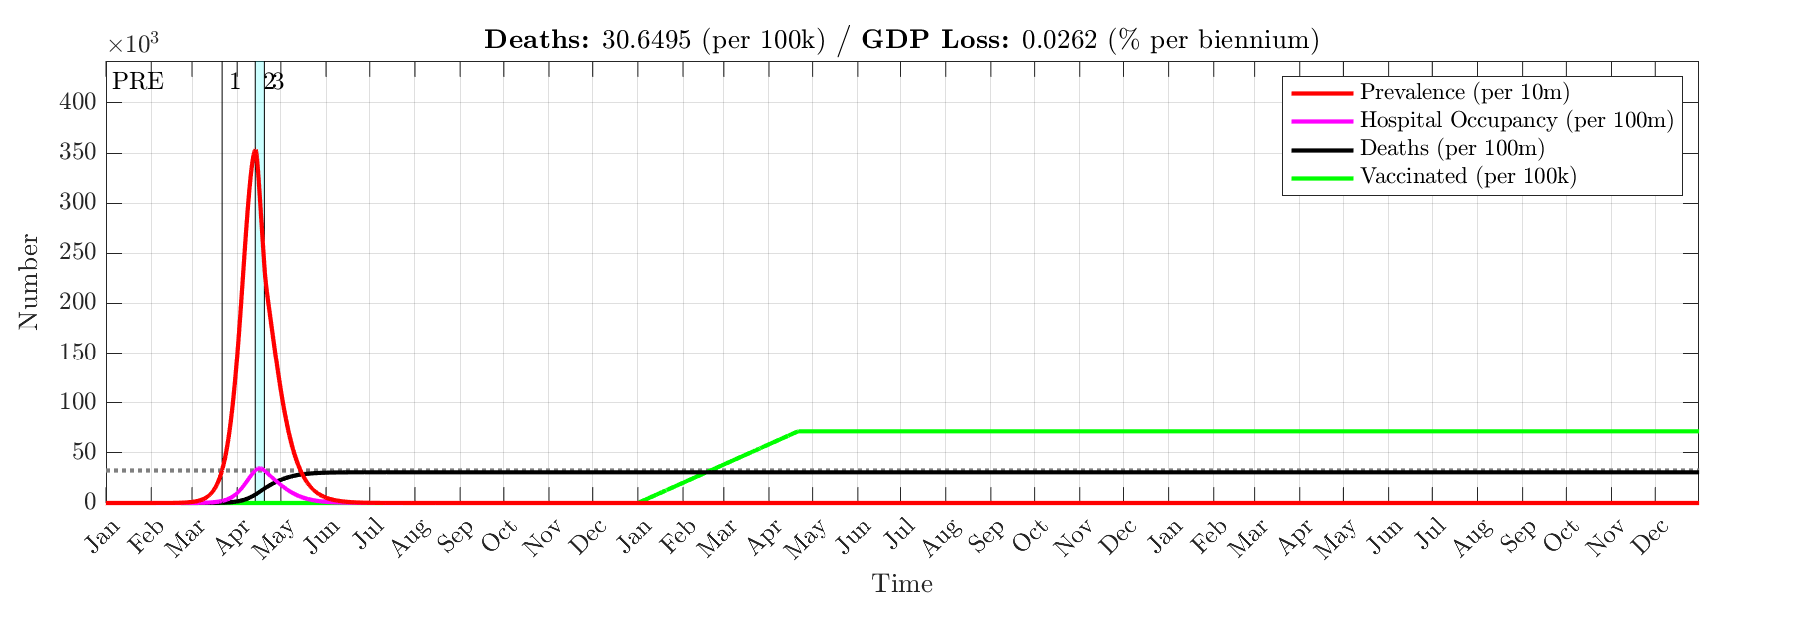
\includegraphics[width=0.95\textwidth,height=5cm]{Unmitigated/Counterfactuals/UK_swfl}}\\
  \sidesubfloat[]{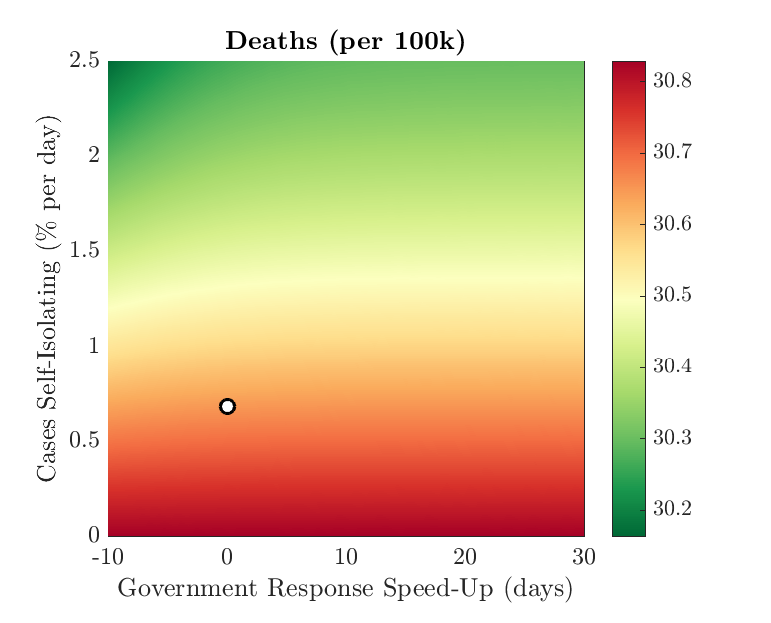
\includegraphics[width=0.40\textwidth,height=5cm]{Unmitigated/UK/SWINE/ero_d}}\hspace{1.8cm}
  \sidesubfloat[]{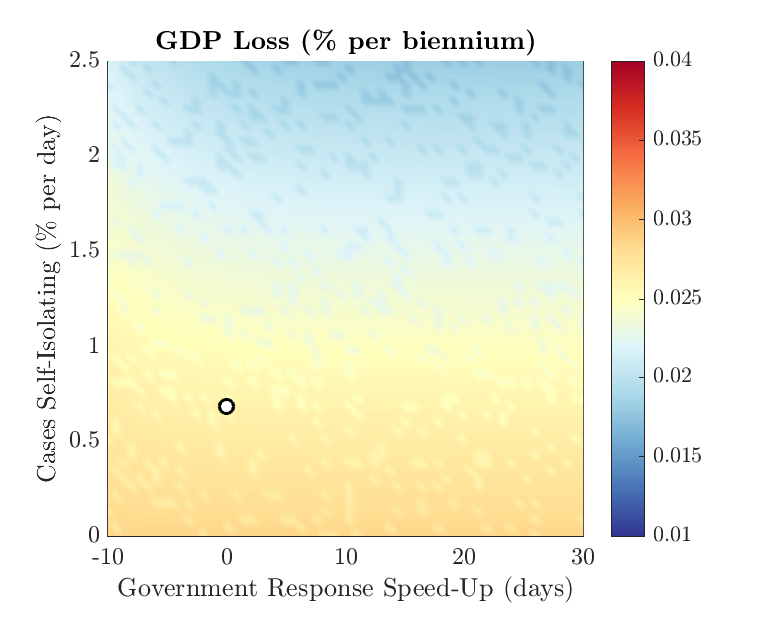
\includegraphics[width=0.40\textwidth,height=5cm]{Unmitigated/UK/SWINE/ero_g}}\\
  \sidesubfloat[]{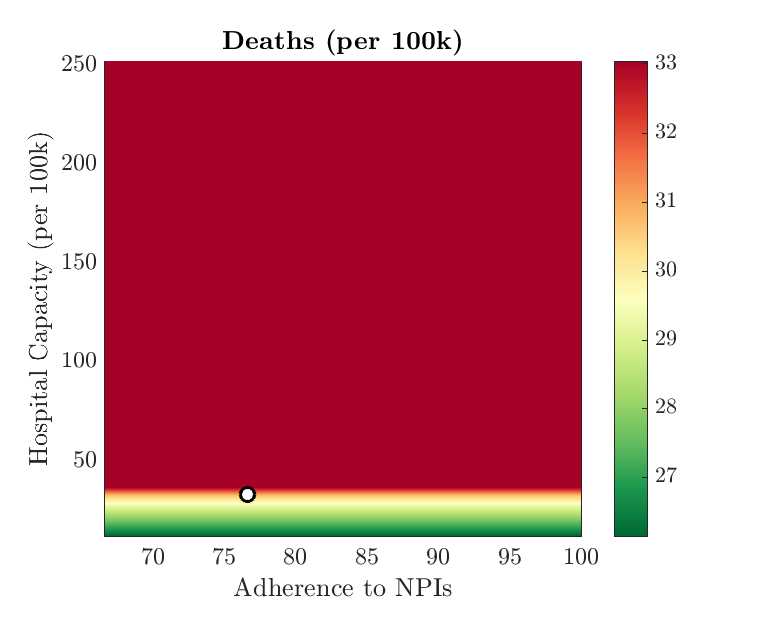
\includegraphics[width=0.40\textwidth,height=5cm]{Unmitigated/UK/SWINE/npl_d}}\hspace{1.8cm}
  \sidesubfloat[]{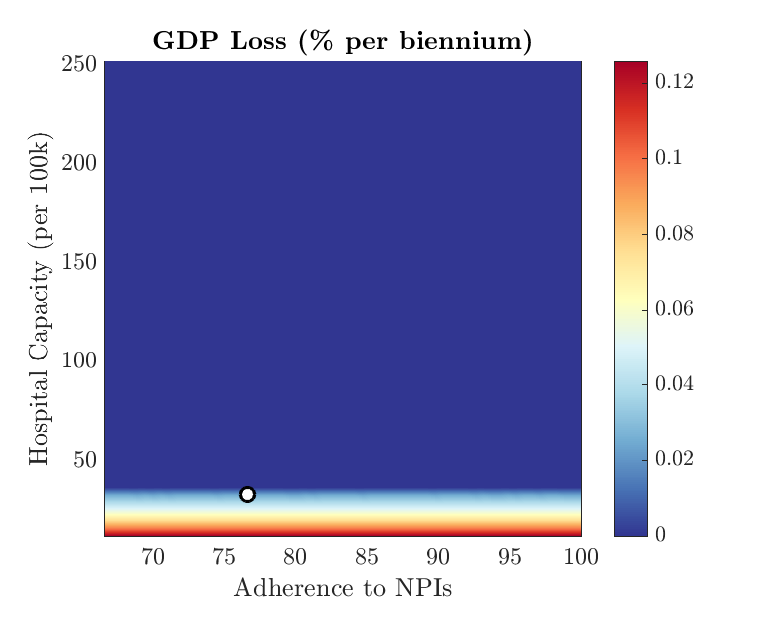
\includegraphics[width=0.40\textwidth,height=5cm]{Unmitigated/UK/SWINE/npl_g}}\\
  \sidesubfloat[]{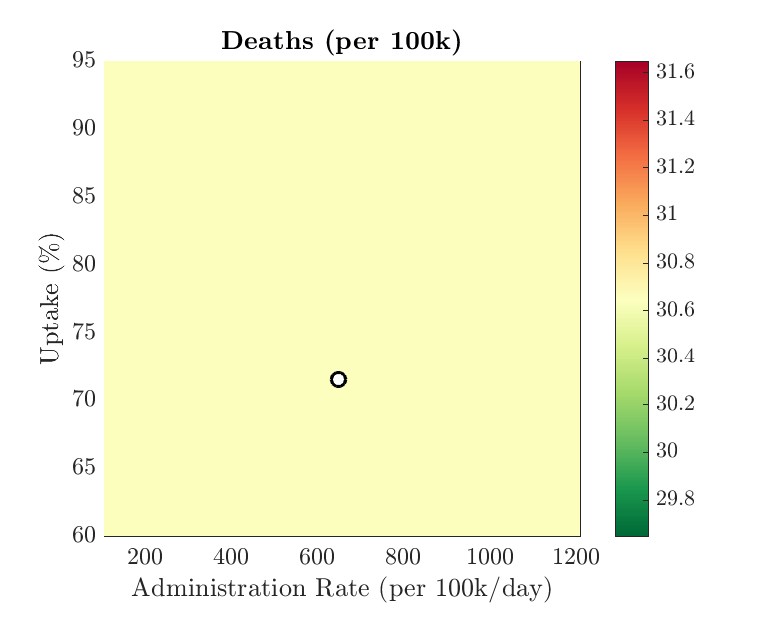
\includegraphics[width=0.40\textwidth,height=5cm]{Unmitigated/UK/SWINE/imm_d}}\hspace{1.76cm}
  \sidesubfloat[]{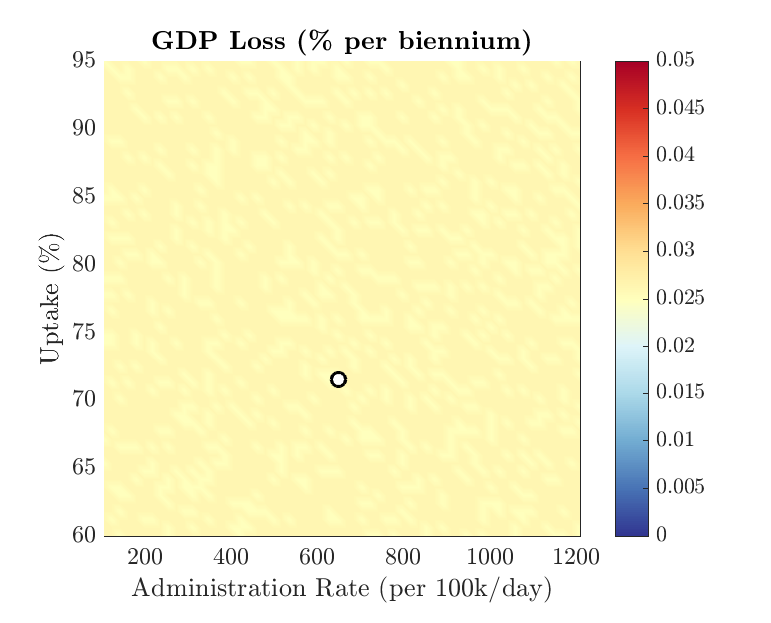
\includegraphics[width=0.40\textwidth,height=5cm]{Unmitigated/UK/SWINE/imm_g}}\\
  \caption*{\textbf{Figure A2:} P2 in the UK; $(a)$ the counterfactual epidemic trajectory; the effects of increasing/decreasing $(b,c)$ the government response time \& proportion of cases self-isolating, $(d,e)$ adherence to NPIs during lockdown \& hospital capacity, and $(f,g)$ vaccine administration rate \& uptake.}
\end{figure}

\begin{figure}[!h]
  \sidesubfloat[]{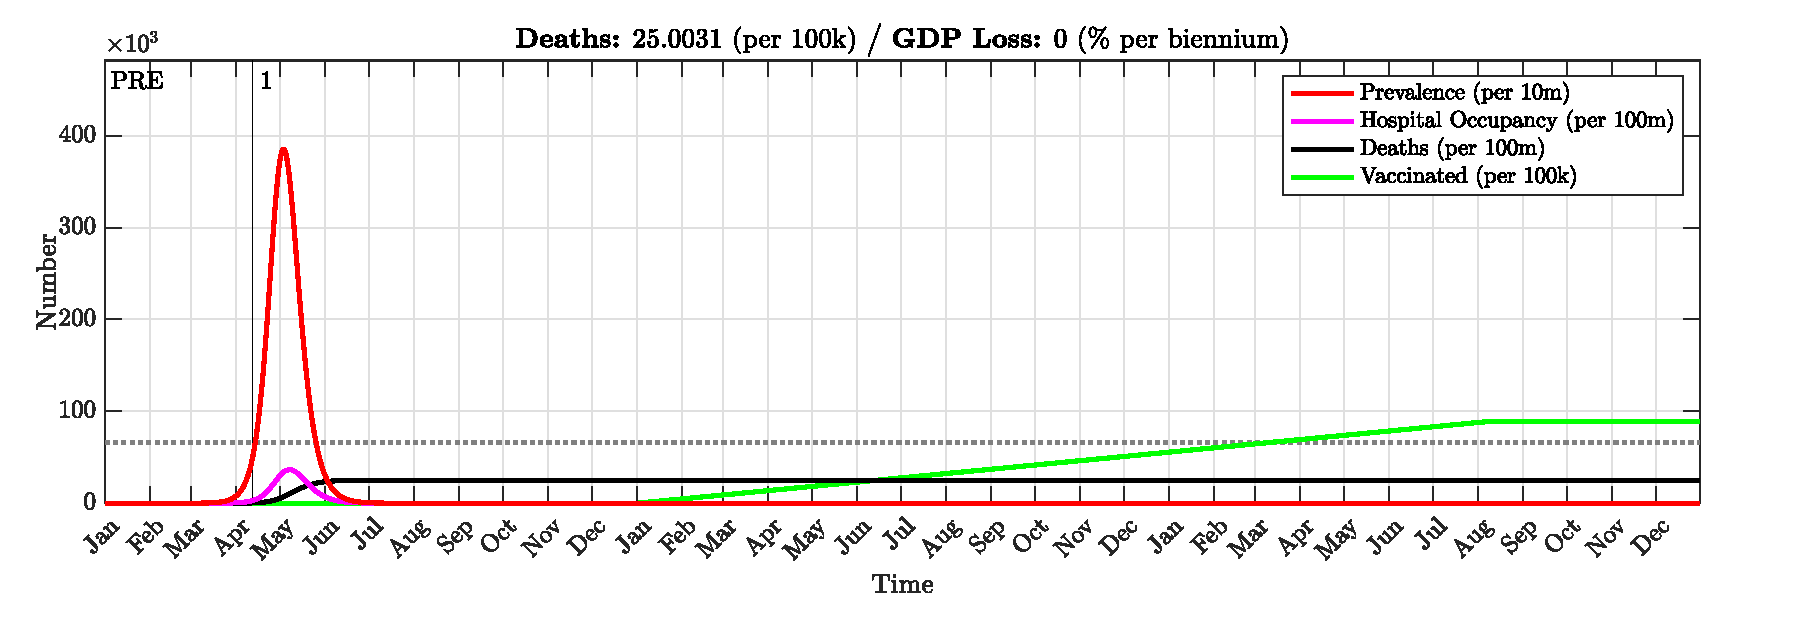
\includegraphics[width=0.95\textwidth,height=5cm]{Unmitigated/Counterfactuals/CN_swfl}}\\
  \sidesubfloat[]{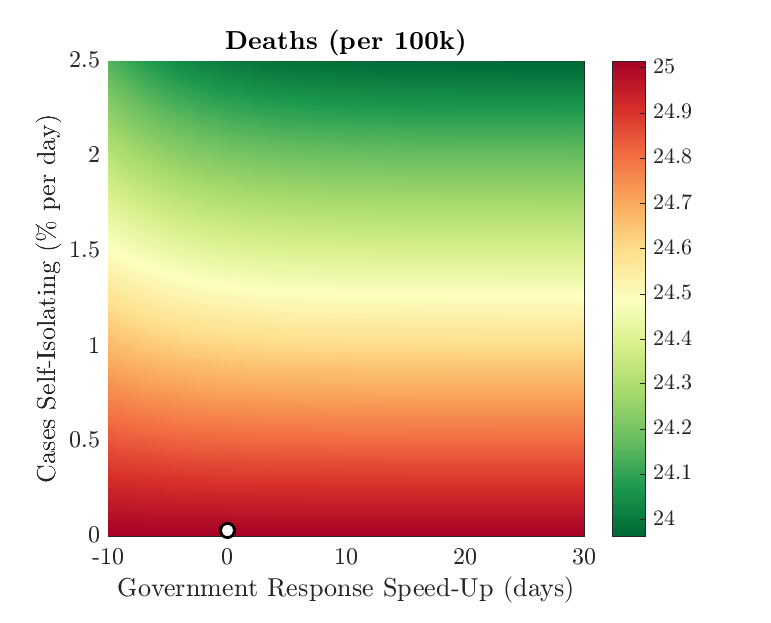
\includegraphics[width=0.40\textwidth,height=5cm]{Unmitigated/CN/SWINE/ero_d}}\hspace{1.8cm}
  \sidesubfloat[]{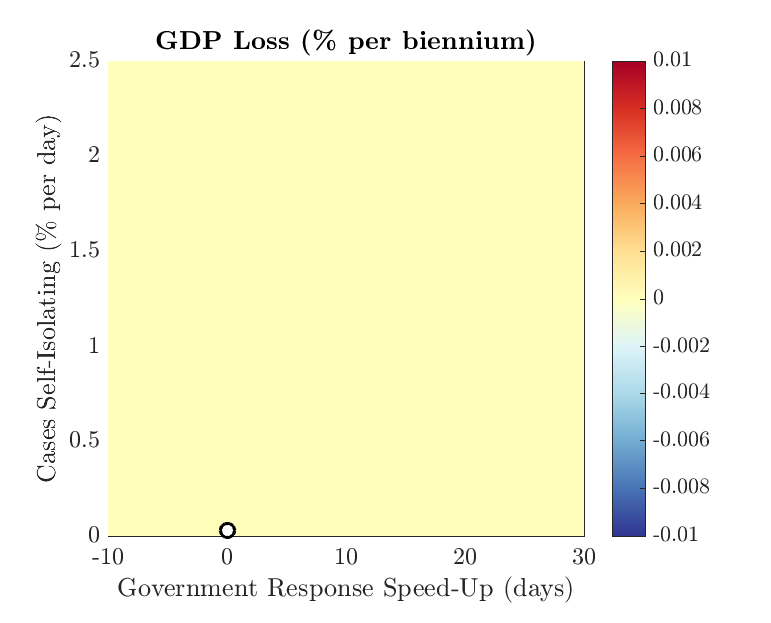
\includegraphics[width=0.40\textwidth,height=5cm]{Unmitigated/CN/SWINE/ero_g}}\\
  \sidesubfloat[]{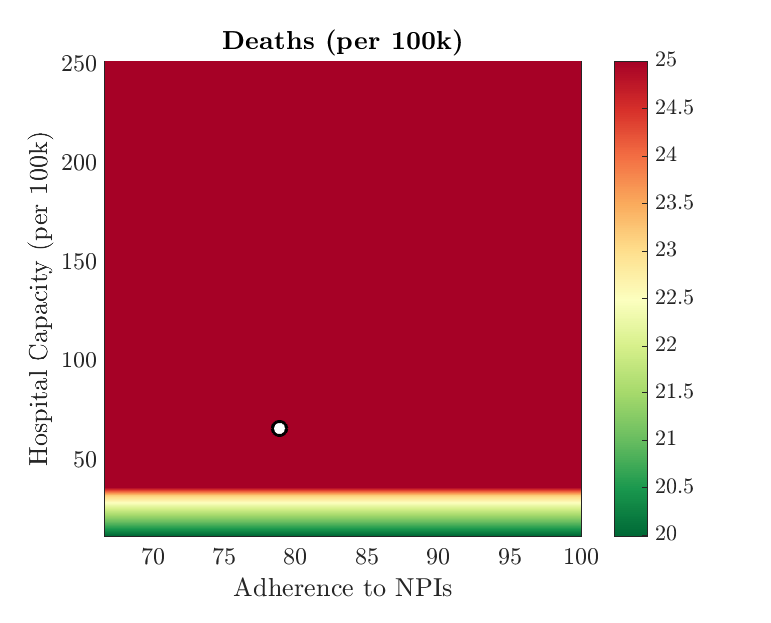
\includegraphics[width=0.40\textwidth,height=5cm]{Unmitigated/CN/SWINE/npl_d}}\hspace{1.8cm}
  \sidesubfloat[]{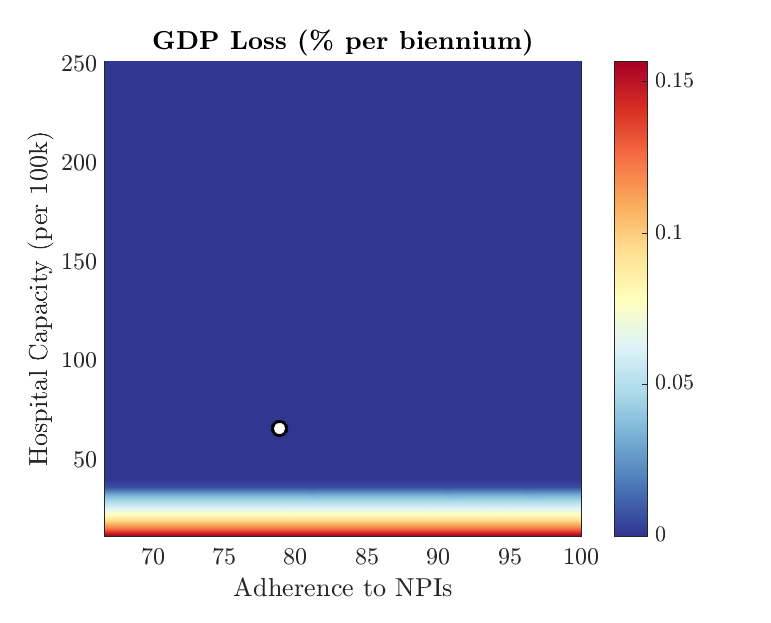
\includegraphics[width=0.40\textwidth,height=5cm]{Unmitigated/CN/SWINE/npl_g}}\\
  \sidesubfloat[]{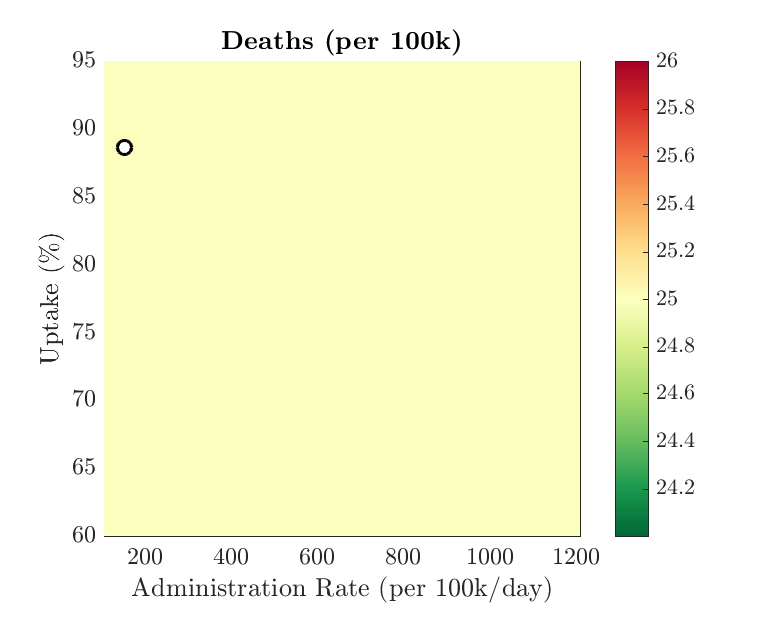
\includegraphics[width=0.40\textwidth,height=5cm]{Unmitigated/CN/SWINE/imm_d}}\hspace{1.76cm}
  \sidesubfloat[]{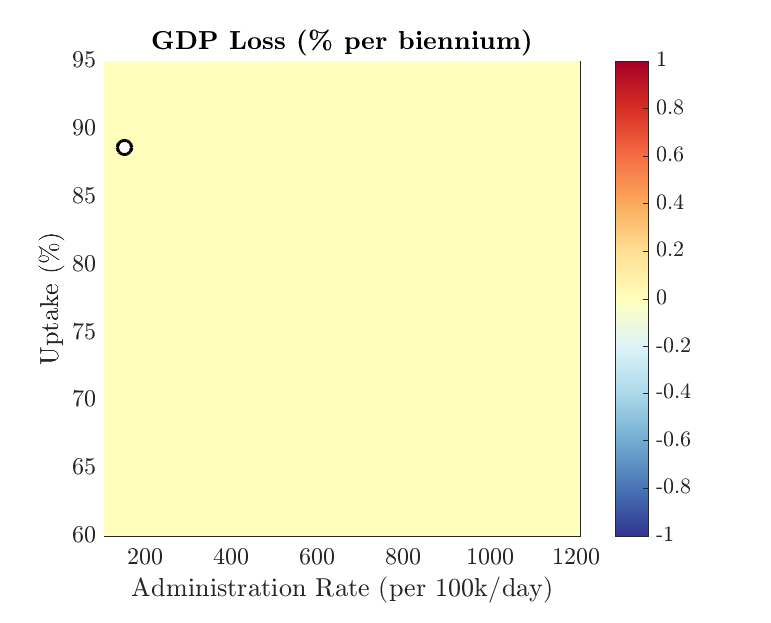
\includegraphics[width=0.40\textwidth,height=5cm]{Unmitigated/CN/SWINE/imm_g}}\\
  \caption*{\textbf{Figure A3:} P2 in China; $(a)$ the counterfactual epidemic trajectory; the effects of increasing/decreasing $(b,c)$ the government response time \& proportion of cases self-isolating, $(d,e)$ adherence to NPIs during lockdown \& hospital capacity, and $(f,g)$ vaccine administration rate \& uptake.}
\end{figure}

\begin{figure}[!h]
  \sidesubfloat[]{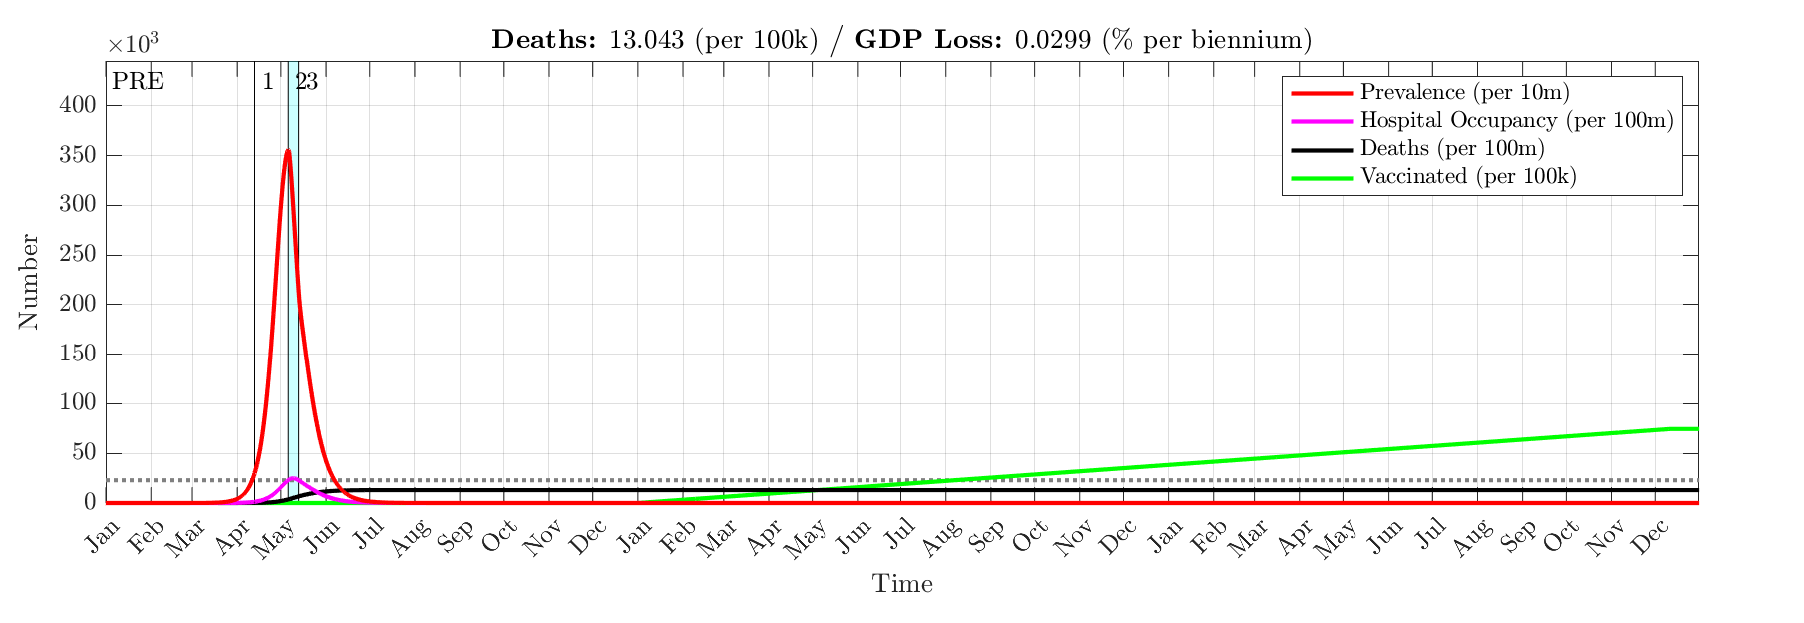
\includegraphics[width=0.95\textwidth,height=5cm]{Unmitigated/Counterfactuals/IN_swfl}}\\
  \sidesubfloat[]{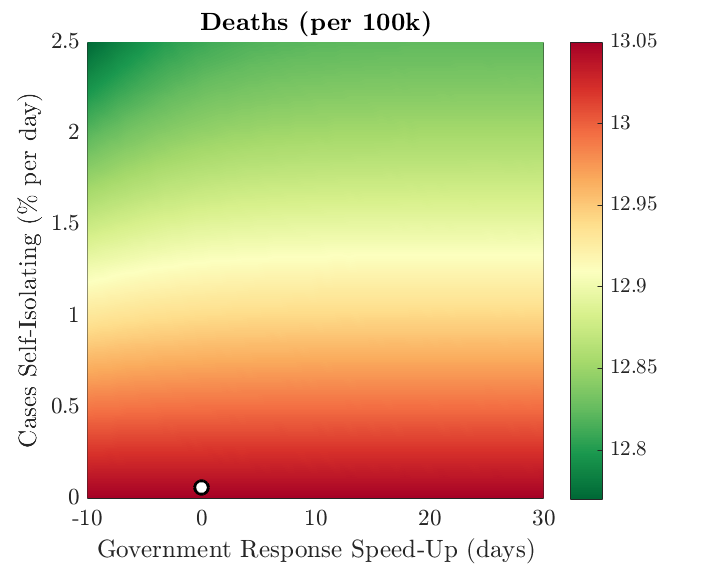
\includegraphics[width=0.40\textwidth,height=5cm]{Unmitigated/IN/SWINE/ero_d}}\hspace{1.8cm}
  \sidesubfloat[]{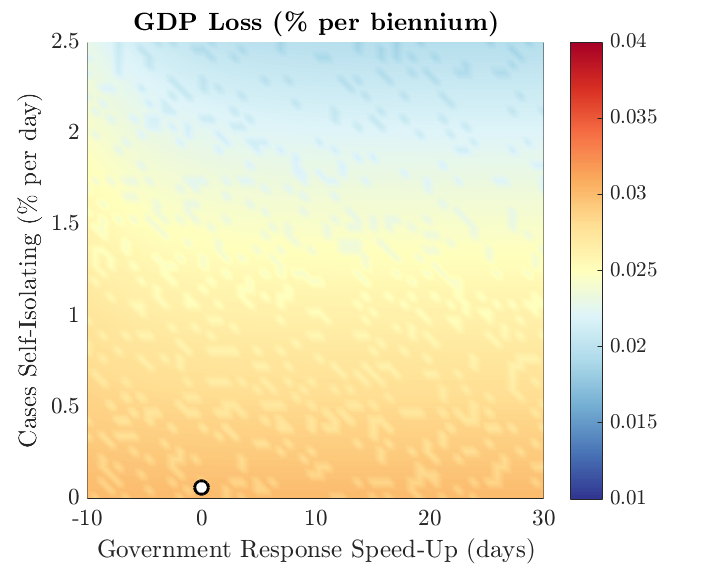
\includegraphics[width=0.40\textwidth,height=5cm]{Unmitigated/IN/SWINE/ero_g}}\\
  \sidesubfloat[]{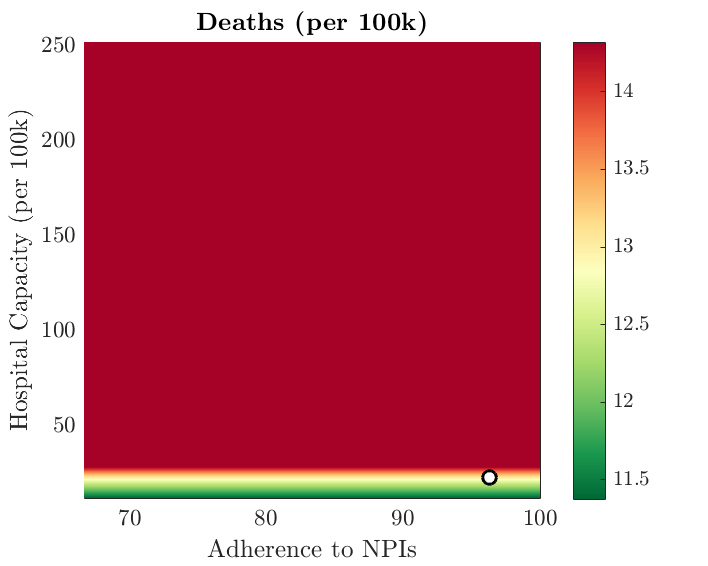
\includegraphics[width=0.40\textwidth,height=5cm]{Unmitigated/IN/SWINE/npl_d}}\hspace{1.8cm}
  \sidesubfloat[]{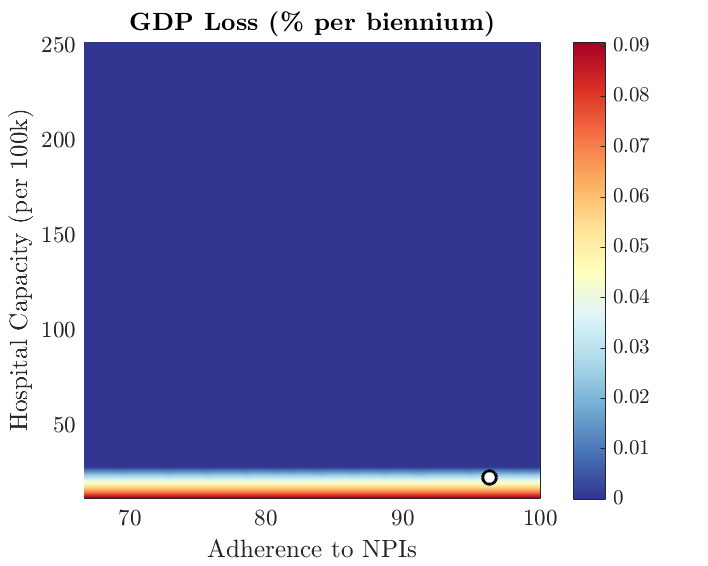
\includegraphics[width=0.40\textwidth,height=5cm]{Unmitigated/IN/SWINE/npl_g}}\\
  \sidesubfloat[]{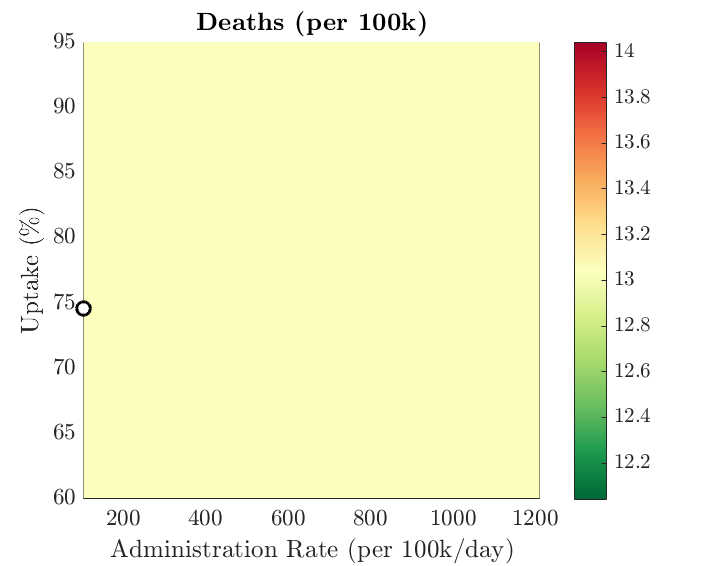
\includegraphics[width=0.40\textwidth,height=5cm]{Unmitigated/IN/SWINE/imm_d}}\hspace{1.76cm}
  \sidesubfloat[]{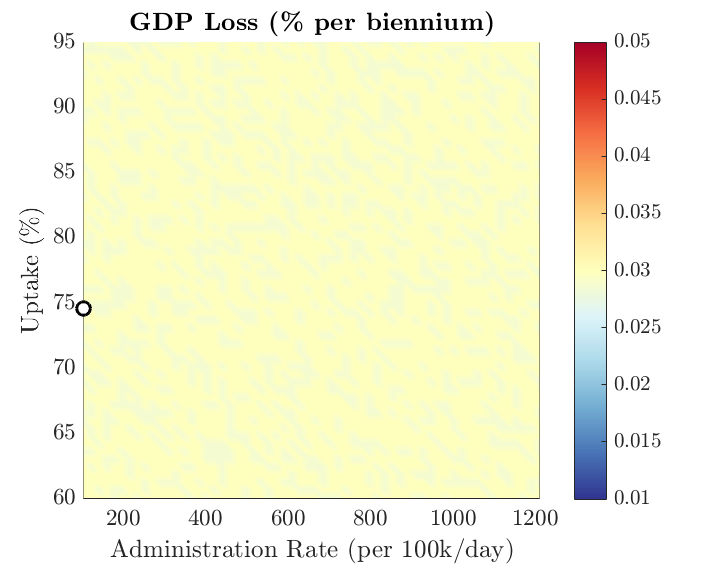
\includegraphics[width=0.40\textwidth,height=5cm]{Unmitigated/IN/SWINE/imm_g}}\\
  \caption*{\textbf{Figure A4:} P2 in India; $(a)$ the counterfactual epidemic trajectory; the effects of increasing/decreasing $(b,c)$ the government response time \& proportion of cases self-isolating, $(d,e)$ adherence to NPIs during lockdown \& hospital capacity, and $(f,g)$ vaccine administration rate \& uptake.}
\end{figure}


\subsection{Spanish Flu}

\begin{figure}[!h]
  \sidesubfloat[]{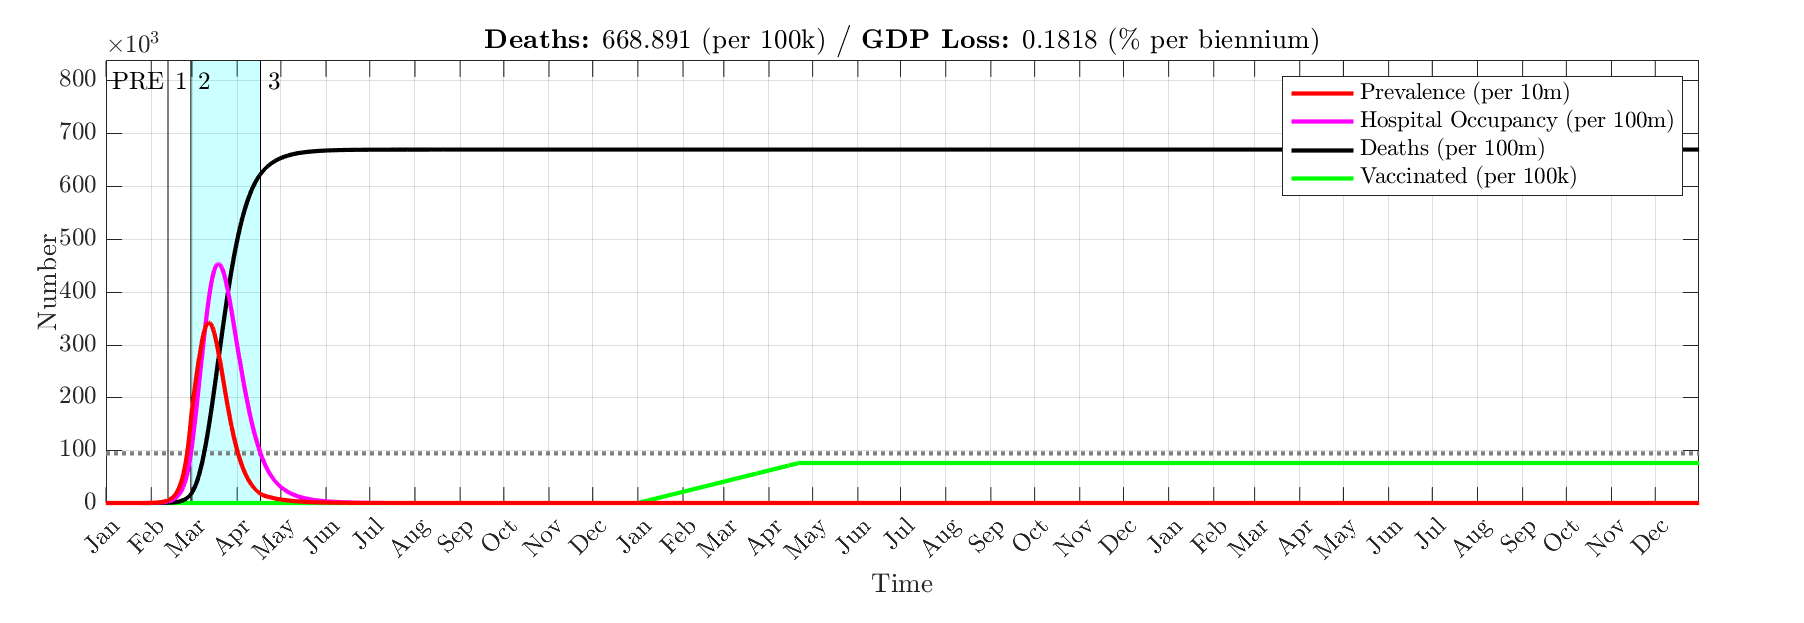
\includegraphics[width=0.95\textwidth,height=5cm]{Unmitigated/Counterfactuals/US_spfl}}\\
  \sidesubfloat[]{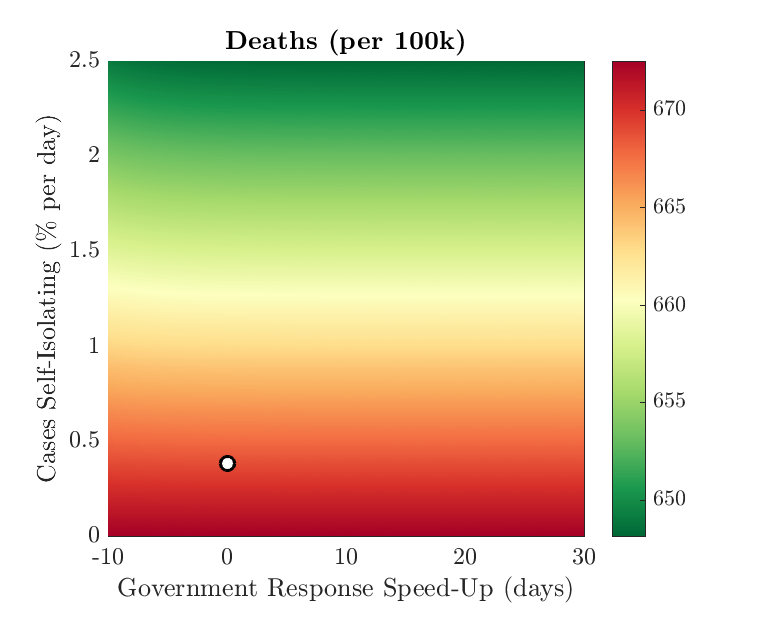
\includegraphics[width=0.40\textwidth,height=5cm]{Unmitigated/US/SPANISH/ero_d}}\hspace{1.8cm}
  \sidesubfloat[]{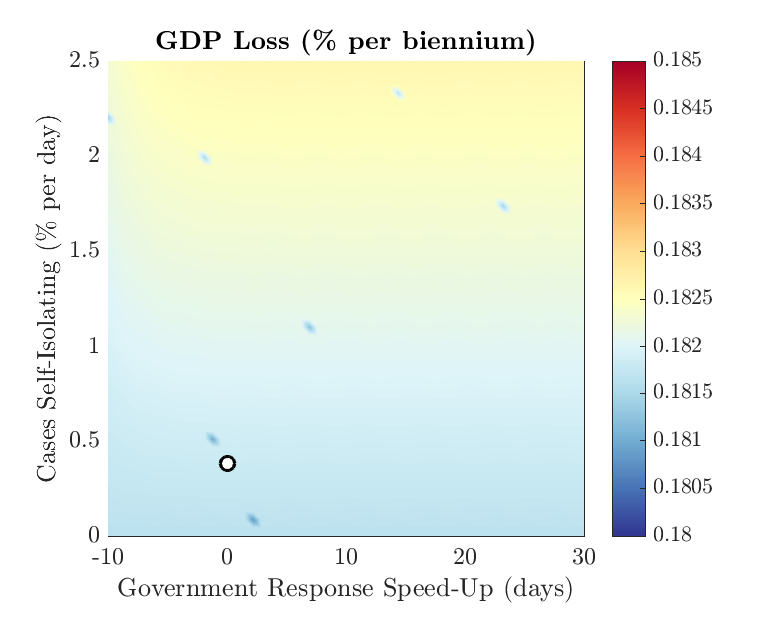
\includegraphics[width=0.40\textwidth,height=5cm]{Unmitigated/US/SPANISH/ero_g}}\\
  \sidesubfloat[]{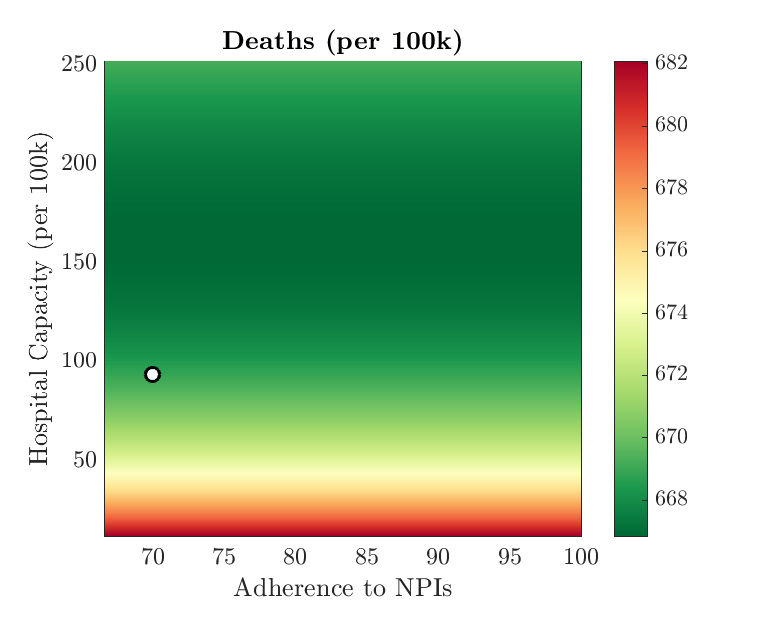
\includegraphics[width=0.40\textwidth,height=5cm]{Unmitigated/US/SPANISH/npl_d}}\hspace{1.8cm}
  \sidesubfloat[]{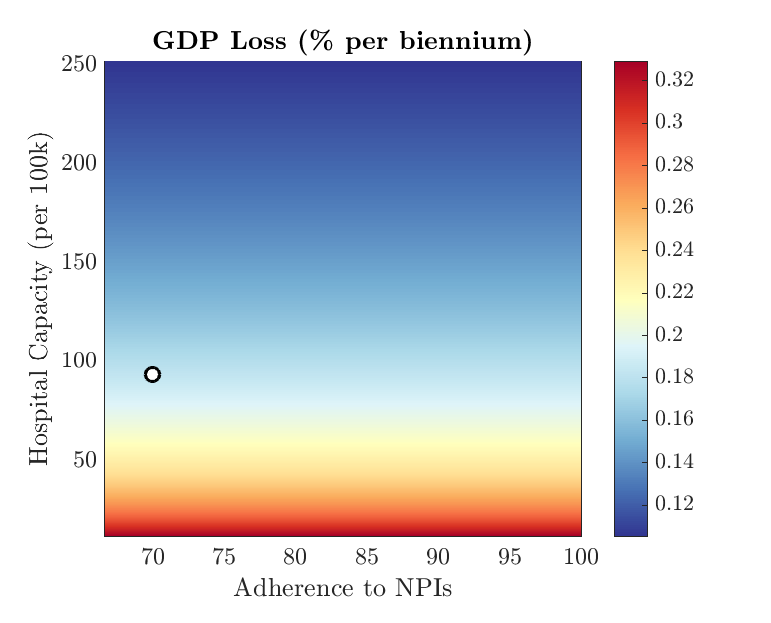
\includegraphics[width=0.40\textwidth,height=5cm]{Unmitigated/US/SPANISH/npl_g}}\\
  \sidesubfloat[]{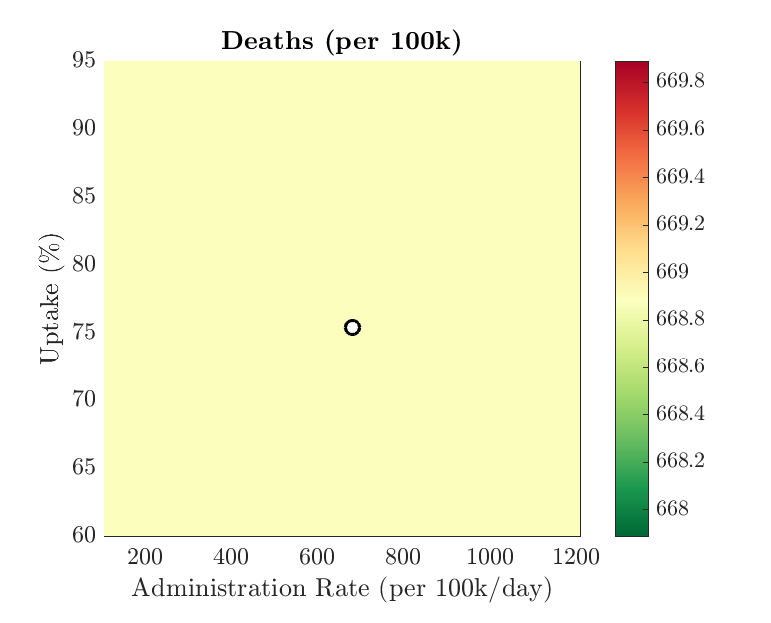
\includegraphics[width=0.40\textwidth,height=5cm]{Unmitigated/US/SPANISH/imm_d}}\hspace{1.76cm}
  \sidesubfloat[]{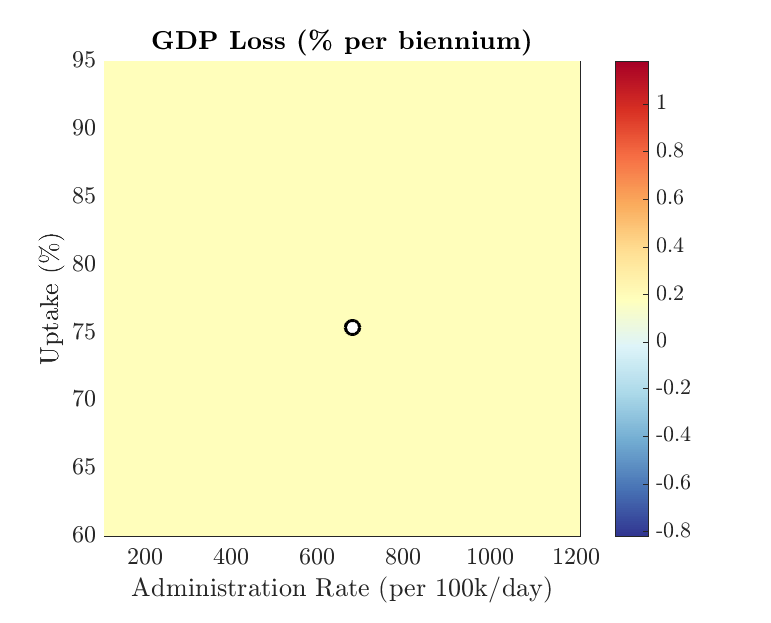
\includegraphics[width=0.40\textwidth,height=5cm]{Unmitigated/US/SPANISH/imm_g}}\\
  \caption*{\textbf{Figure A5:} P2 in the USA; $(a)$ the counterfactual epidemic trajectory; the effects of increasing/decreasing $(b,c)$ the government response time \& proportion of cases self-isolating, $(d,e)$ adherence to NPIs during lockdown \& hospital capacity, and $(f,g)$ vaccine administration rate \& uptake.}
\end{figure}

\begin{figure}[!h]
  \sidesubfloat[]{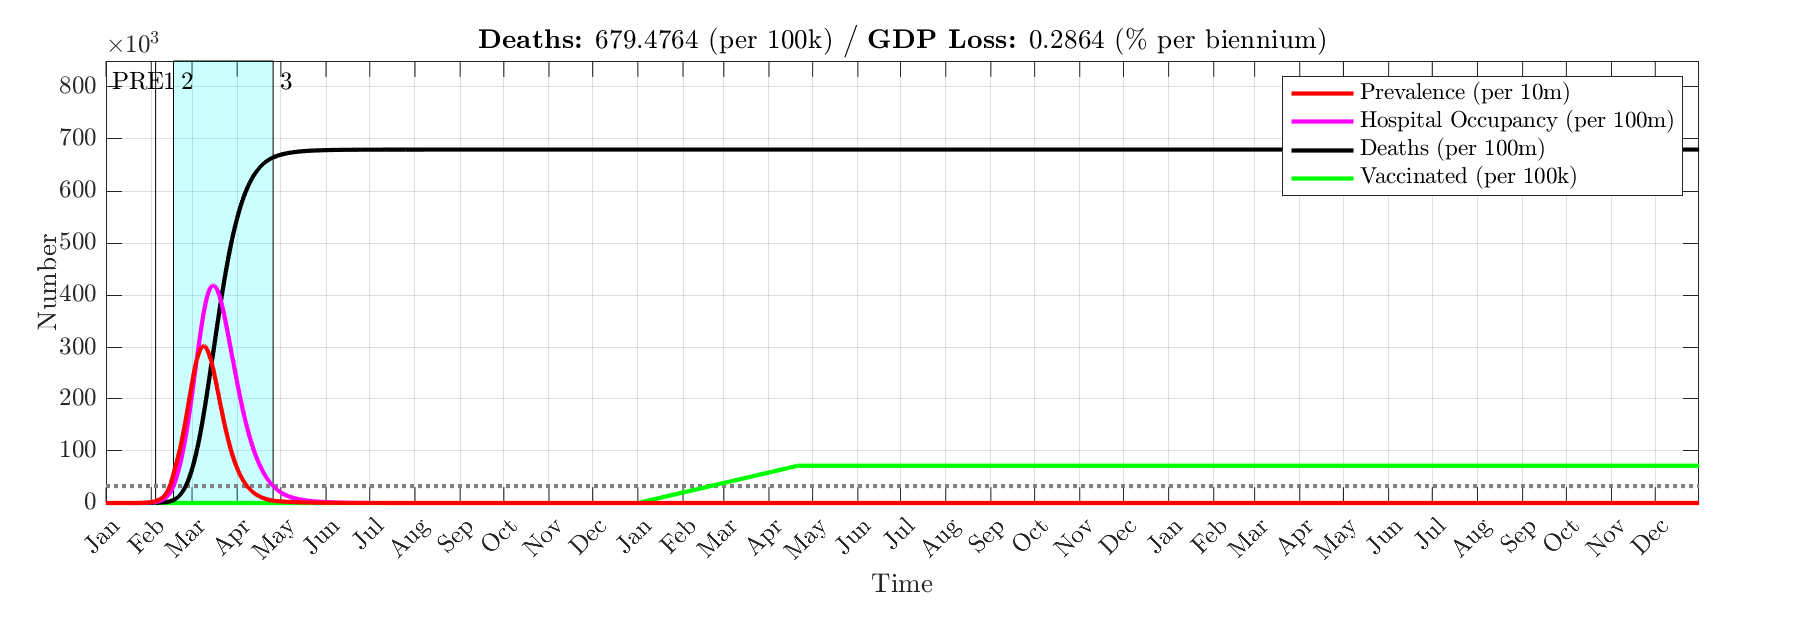
\includegraphics[width=0.95\textwidth,height=5cm]{Unmitigated/Counterfactuals/UK_spfl}}\\
  \sidesubfloat[]{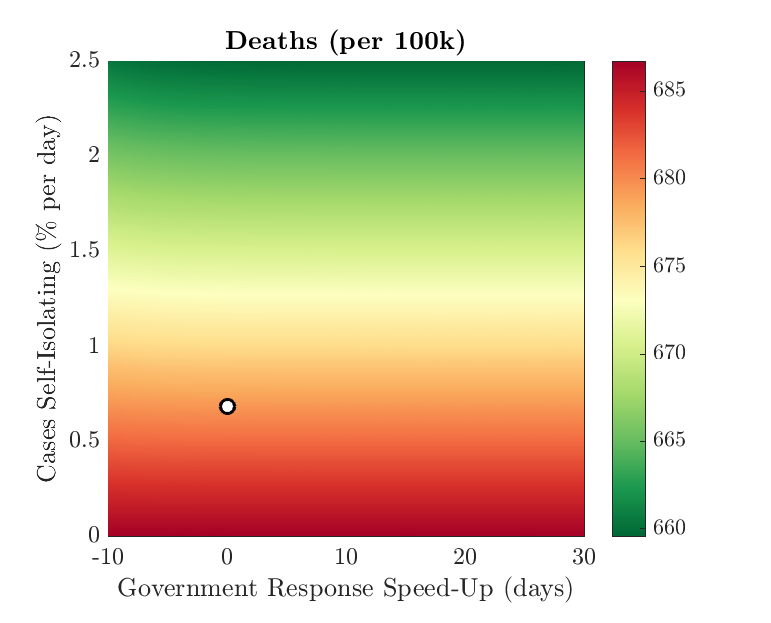
\includegraphics[width=0.40\textwidth,height=5cm]{Unmitigated/UK/SPANISH/ero_d}}\hspace{1.8cm}
  \sidesubfloat[]{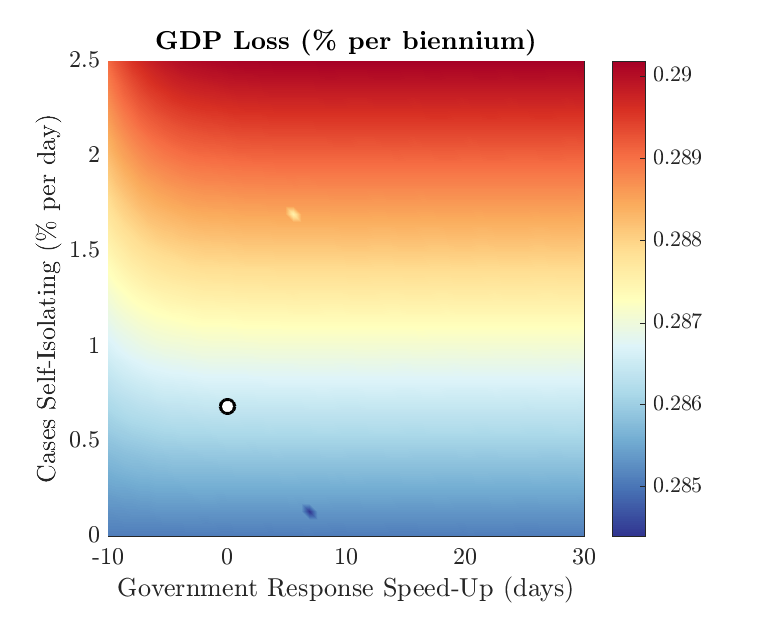
\includegraphics[width=0.40\textwidth,height=5cm]{Unmitigated/UK/SPANISH/ero_g}}\\
  \sidesubfloat[]{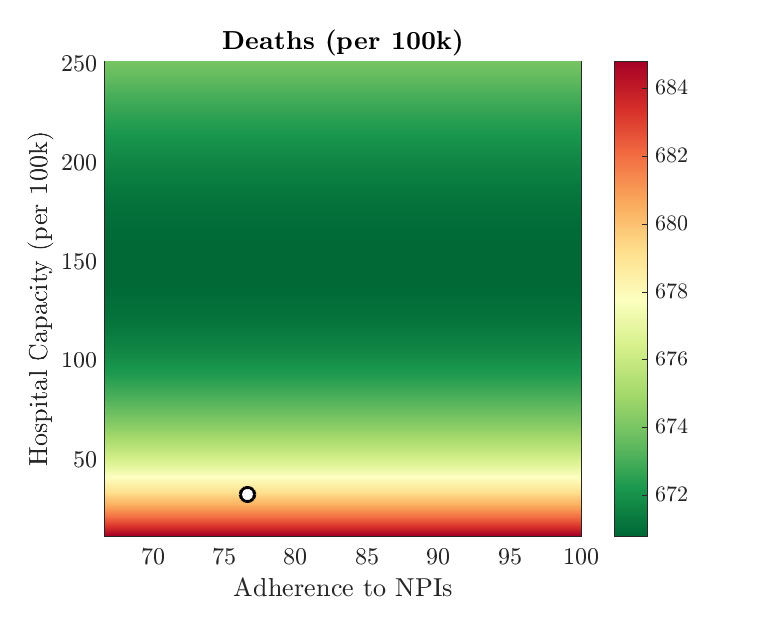
\includegraphics[width=0.40\textwidth,height=5cm]{Unmitigated/UK/SPANISH/npl_d}}\hspace{1.8cm}
  \sidesubfloat[]{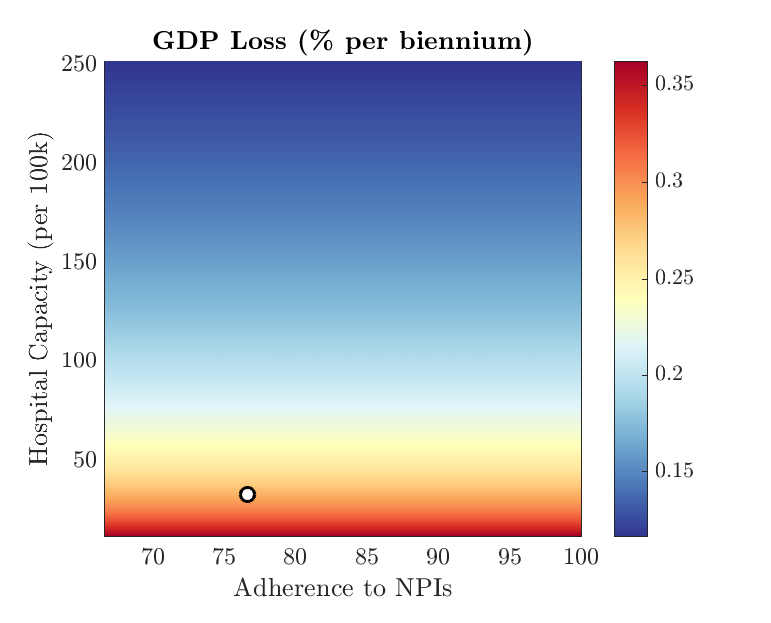
\includegraphics[width=0.40\textwidth,height=5cm]{Unmitigated/UK/SPANISH/npl_g}}\\
  \sidesubfloat[]{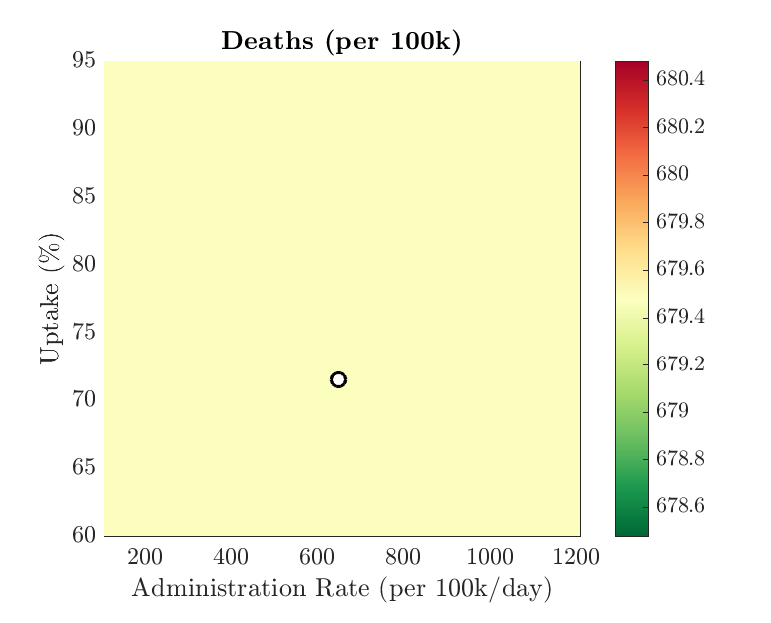
\includegraphics[width=0.40\textwidth,height=5cm]{Unmitigated/UK/SPANISH/imm_d}}\hspace{1.76cm}
  \sidesubfloat[]{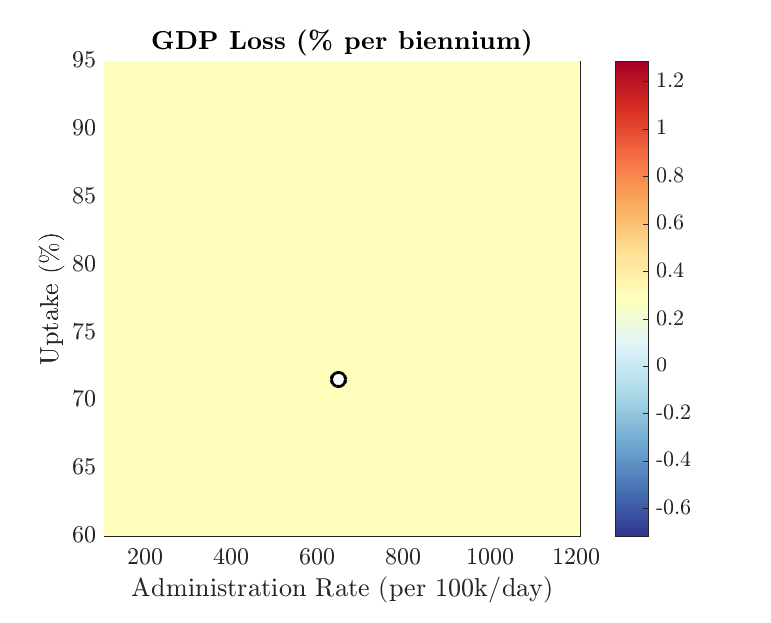
\includegraphics[width=0.40\textwidth,height=5cm]{Unmitigated/UK/SPANISH/imm_g}}\\
  \caption*{\textbf{Figure A6:} P2 in the UK; $(a)$ the counterfactual epidemic trajectory; the effects of increasing/decreasing $(b,c)$ the government response time \& proportion of cases self-isolating, $(d,e)$ adherence to NPIs during lockdown \& hospital capacity, and $(f,g)$ vaccine administration rate \& uptake.}
\end{figure}

\begin{figure}[!h]
  \sidesubfloat[]{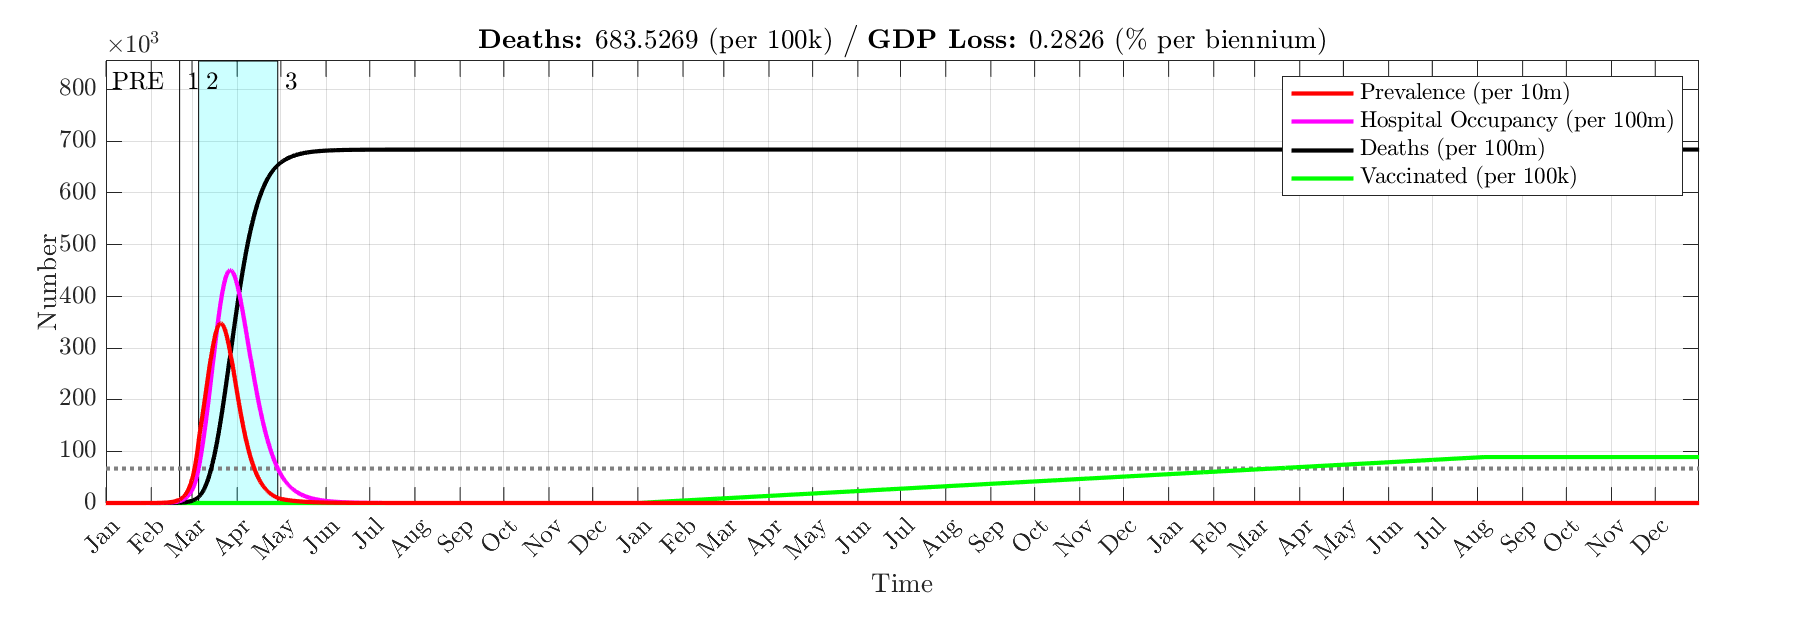
\includegraphics[width=0.95\textwidth,height=5cm]{Unmitigated/Counterfactuals/CN_spfl}}\\
  \sidesubfloat[]{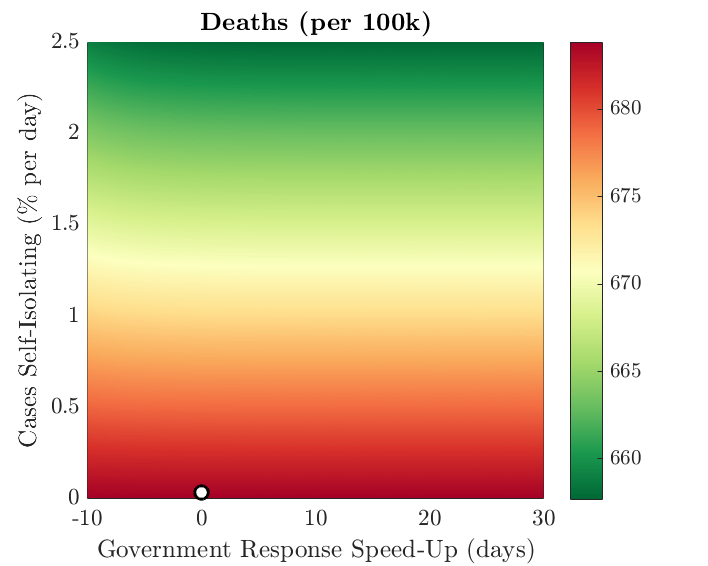
\includegraphics[width=0.40\textwidth,height=5cm]{Unmitigated/CN/SPANISH/ero_d}}\hspace{1.8cm}
  \sidesubfloat[]{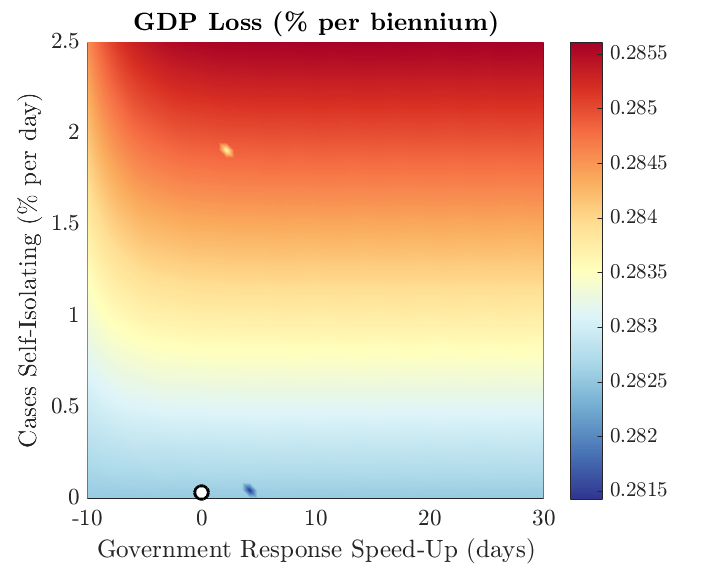
\includegraphics[width=0.40\textwidth,height=5cm]{Unmitigated/CN/SPANISH/ero_g}}\\
  \sidesubfloat[]{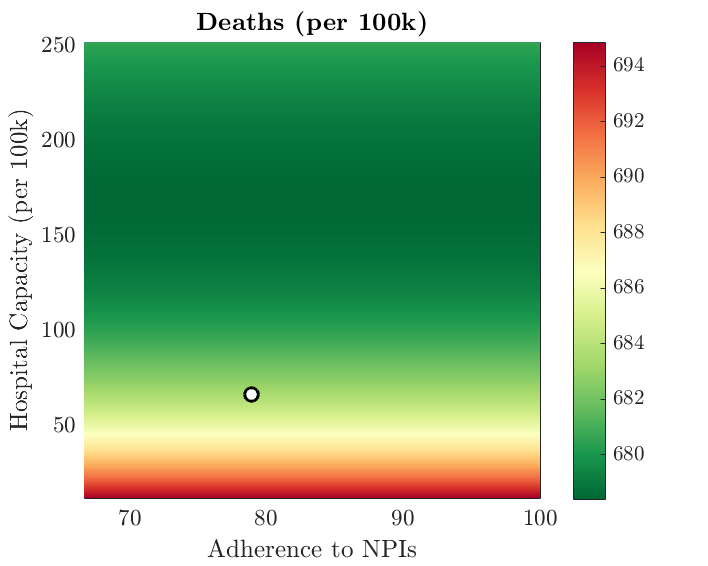
\includegraphics[width=0.40\textwidth,height=5cm]{Unmitigated/CN/SPANISH/npl_d}}\hspace{1.8cm}
  \sidesubfloat[]{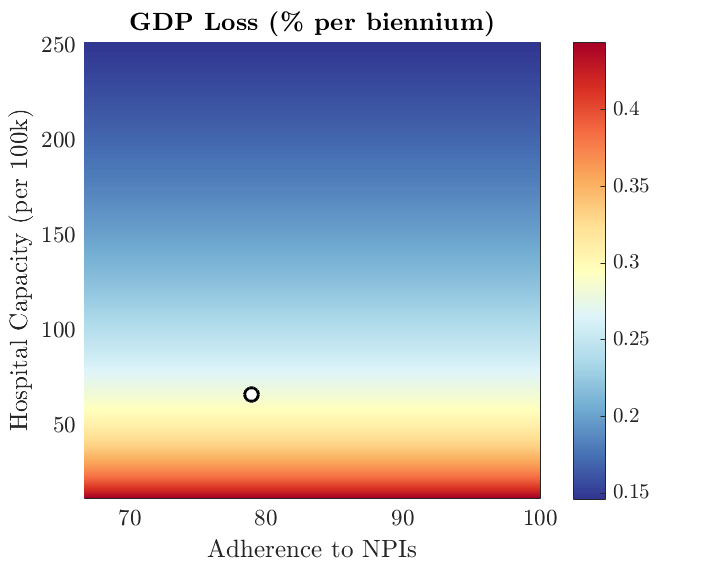
\includegraphics[width=0.40\textwidth,height=5cm]{Unmitigated/CN/SPANISH/npl_g}}\\
  \sidesubfloat[]{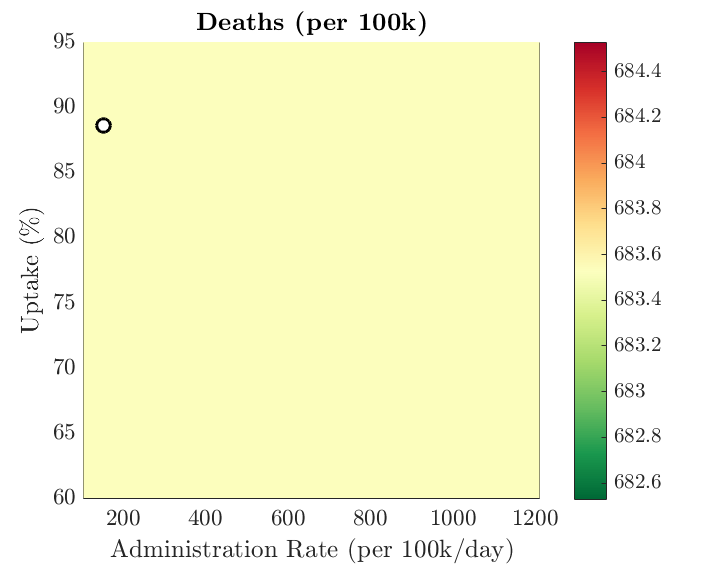
\includegraphics[width=0.40\textwidth,height=5cm]{Unmitigated/CN/SPANISH/imm_d}}\hspace{1.76cm}
  \sidesubfloat[]{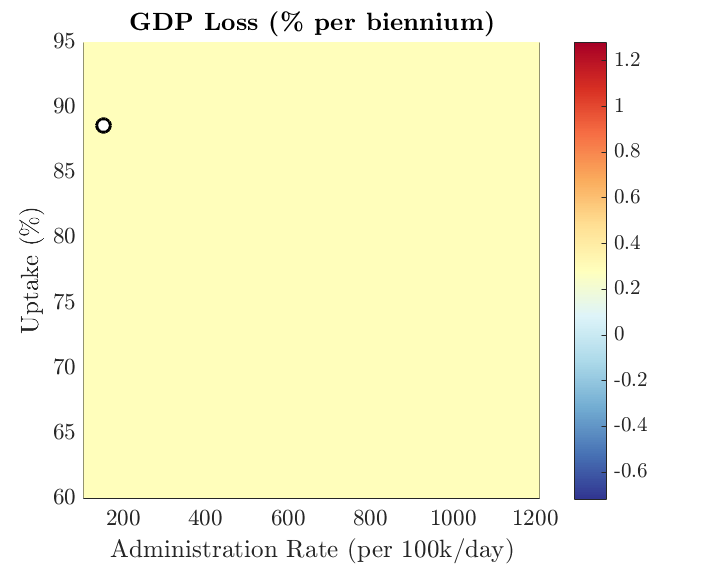
\includegraphics[width=0.40\textwidth,height=5cm]{Unmitigated/CN/SPANISH/imm_g}}\\
  \caption*{\textbf{Figure A7:} P2 in China; $(a)$ the counterfactual epidemic trajectory; the effects of increasing/decreasing $(b,c)$ the government response time \& proportion of cases self-isolating, $(d,e)$ adherence to NPIs during lockdown \& hospital capacity, and $(f,g)$ vaccine administration rate \& uptake.}
\end{figure}

\begin{figure}[!h]
  \sidesubfloat[]{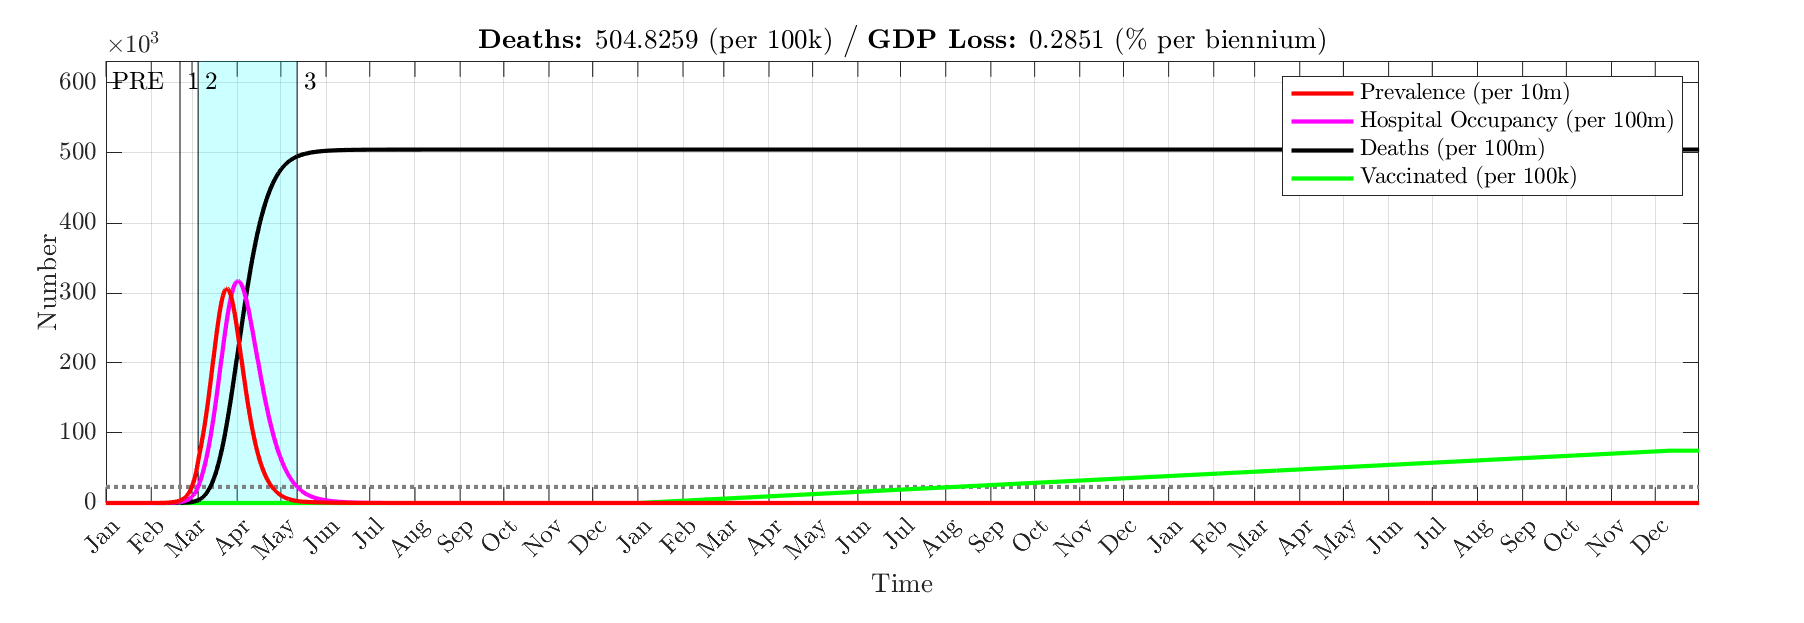
\includegraphics[width=0.95\textwidth,height=5cm]{Unmitigated/Counterfactuals/IN_spfl}}\\
  \sidesubfloat[]{\includegraphics[width=0.40\textwidth,height=5cm]{Unmitigated/IN/SPANISH/ero_d}}\hspace{1.8cm}
  \sidesubfloat[]{\includegraphics[width=0.40\textwidth,height=5cm]{Unmitigated/IN/SPANISH/ero_g}}\\
  \sidesubfloat[]{\includegraphics[width=0.40\textwidth,height=5cm]{Unmitigated/IN/SPANISH/npl_d}}\hspace{1.8cm}
  \sidesubfloat[]{\includegraphics[width=0.40\textwidth,height=5cm]{Unmitigated/IN/SPANISH/npl_g}}\\
  \sidesubfloat[]{\includegraphics[width=0.40\textwidth,height=5cm]{Unmitigated/IN/SPANISH/imm_d}}\hspace{1.76cm}
  \sidesubfloat[]{\includegraphics[width=0.40\textwidth,height=5cm]{Unmitigated/IN/SPANISH/imm_g}}\\
  \caption*{\textbf{Figure A8:} P2 in India; $(a)$ the counterfactual epidemic trajectory; the effects of increasing/decreasing $(b,c)$ the government response time \& proportion of cases self-isolating, $(d,e)$ adherence to NPIs during lockdown \& hospital capacity, and $(f,g)$ vaccine administration rate \& uptake.}
\end{figure}


\subsection{Covid}

\begin{figure}[!h]
  \sidesubfloat[]{\includegraphics[width=0.95\textwidth,height=5cm]{Unmitigated/Counterfactuals/US_cv19}}\\
  \sidesubfloat[]{\includegraphics[width=0.40\textwidth,height=5cm]{Unmitigated/US/COVID/ero_d}}\hspace{1.8cm}
  \sidesubfloat[]{\includegraphics[width=0.40\textwidth,height=5cm]{Unmitigated/US/COVID/ero_g}}\\
  \sidesubfloat[]{\includegraphics[width=0.40\textwidth,height=5cm]{Unmitigated/US/COVID/npl_d}}\hspace{1.8cm}
  \sidesubfloat[]{\includegraphics[width=0.40\textwidth,height=5cm]{Unmitigated/US/COVID/npl_g}}\\
  \sidesubfloat[]{\includegraphics[width=0.40\textwidth,height=5cm]{Unmitigated/US/COVID/imm_d}}\hspace{1.76cm}
  \sidesubfloat[]{\includegraphics[width=0.40\textwidth,height=5cm]{Unmitigated/US/COVID/imm_g}}\\
  \caption*{\textbf{Figure A9:} P2 in the USA; $(a)$ the counterfactual epidemic trajectory; the effects of increasing/decreasing $(b,c)$ the government response time \& proportion of cases self-isolating, $(d,e)$ adherence to NPIs during lockdown \& hospital capacity, and $(f,g)$ vaccine administration rate \& uptake.}
\end{figure}

\begin{figure}[!h]
  \sidesubfloat[]{\includegraphics[width=0.95\textwidth,height=5cm]{Unmitigated/Counterfactuals/UK_cv19}}\\
  \sidesubfloat[]{\includegraphics[width=0.40\textwidth,height=5cm]{Unmitigated/UK/COVID/ero_d}}\hspace{1.8cm}
  \sidesubfloat[]{\includegraphics[width=0.40\textwidth,height=5cm]{Unmitigated/UK/COVID/ero_g}}\\
  \sidesubfloat[]{\includegraphics[width=0.40\textwidth,height=5cm]{Unmitigated/UK/COVID/npl_d}}\hspace{1.8cm}
  \sidesubfloat[]{\includegraphics[width=0.40\textwidth,height=5cm]{Unmitigated/UK/COVID/npl_g}}\\
  \sidesubfloat[]{\includegraphics[width=0.40\textwidth,height=5cm]{Unmitigated/UK/COVID/imm_d}}\hspace{1.76cm}
  \sidesubfloat[]{\includegraphics[width=0.40\textwidth,height=5cm]{Unmitigated/UK/COVID/imm_g}}\\
  \caption*{\textbf{Figure A10:} P2 in the UK; $(a)$ the counterfactual epidemic trajectory; the effects of increasing/decreasing $(b,c)$ the government response time \& proportion of cases self-isolating, $(d,e)$ adherence to NPIs during lockdown \& hospital capacity, and $(f,g)$ vaccine administration rate \& uptake.}
\end{figure}

\begin{figure}[!h]
  \sidesubfloat[]{\includegraphics[width=0.95\textwidth,height=5cm]{Unmitigated/Counterfactuals/CN_cv19}}\\
  \sidesubfloat[]{\includegraphics[width=0.40\textwidth,height=5cm]{Unmitigated/CN/COVID/ero_d}}\hspace{1.8cm}
  \sidesubfloat[]{\includegraphics[width=0.40\textwidth,height=5cm]{Unmitigated/CN/COVID/ero_g}}\\
  \sidesubfloat[]{\includegraphics[width=0.40\textwidth,height=5cm]{Unmitigated/CN/COVID/npl_d}}\hspace{1.8cm}
  \sidesubfloat[]{\includegraphics[width=0.40\textwidth,height=5cm]{Unmitigated/CN/COVID/npl_g}}\\
  \sidesubfloat[]{\includegraphics[width=0.40\textwidth,height=5cm]{Unmitigated/CN/COVID/imm_d}}\hspace{1.76cm}
  \sidesubfloat[]{\includegraphics[width=0.40\textwidth,height=5cm]{Unmitigated/CN/COVID/imm_g}}\\
  \caption*{\textbf{Figure A11:} P2 in China; $(a)$ the counterfactual epidemic trajectory; the effects of increasing/decreasing $(b,c)$ the government response time \& proportion of cases self-isolating, $(d,e)$ adherence to NPIs during lockdown \& hospital capacity, and $(f,g)$ vaccine administration rate \& uptake.}
\end{figure}

\begin{figure}[!h]
  \sidesubfloat[]{\includegraphics[width=0.95\textwidth,height=5cm]{Unmitigated/Counterfactuals/IN_cv19}}\\
  \sidesubfloat[]{\includegraphics[width=0.40\textwidth,height=5cm]{Unmitigated/IN/COVID/ero_d}}\hspace{1.8cm}
  \sidesubfloat[]{\includegraphics[width=0.40\textwidth,height=5cm]{Unmitigated/IN/COVID/ero_g}}\\
  \sidesubfloat[]{\includegraphics[width=0.40\textwidth,height=5cm]{Unmitigated/IN/COVID/npl_d}}\hspace{1.8cm}
  \sidesubfloat[]{\includegraphics[width=0.40\textwidth,height=5cm]{Unmitigated/IN/COVID/npl_g}}\\
  \sidesubfloat[]{\includegraphics[width=0.40\textwidth,height=5cm]{Unmitigated/IN/COVID/imm_d}}\hspace{1.76cm}
  \sidesubfloat[]{\includegraphics[width=0.40\textwidth,height=5cm]{Unmitigated/IN/COVID/imm_g}}\\
  \caption*{\textbf{Figure A12:} P2 in India; $(a)$ the counterfactual epidemic trajectory; the effects of increasing/decreasing $(b,c)$ the government response time \& proportion of cases self-isolating, $(d,e)$ adherence to NPIs during lockdown \& hospital capacity, and $(f,g)$ vaccine administration rate \& uptake.}
\end{figure}


\subsection{SARS}

\begin{figure}[!h]
  \sidesubfloat[]{\includegraphics[width=0.95\textwidth,height=5cm]{Unmitigated/Counterfactuals/US_sars}}\\
  \sidesubfloat[]{\includegraphics[width=0.40\textwidth,height=5cm]{Unmitigated/US/SARS/ero_d}}\hspace{1.8cm}
  \sidesubfloat[]{\includegraphics[width=0.40\textwidth,height=5cm]{Unmitigated/US/SARS/ero_g}}\\
  \sidesubfloat[]{\includegraphics[width=0.40\textwidth,height=5cm]{Unmitigated/US/SARS/npl_d}}\hspace{1.8cm}
  \sidesubfloat[]{\includegraphics[width=0.40\textwidth,height=5cm]{Unmitigated/US/SARS/npl_g}}\\
  \sidesubfloat[]{\includegraphics[width=0.40\textwidth,height=5cm]{Unmitigated/US/SARS/imm_d}}\hspace{1.76cm}
  \sidesubfloat[]{\includegraphics[width=0.40\textwidth,height=5cm]{Unmitigated/US/SARS/imm_g}}\\
  \caption*{\textbf{Figure A13:} P2 in the USA; $(a)$ the counterfactual epidemic trajectory; the effects of increasing/decreasing $(b,c)$ the government response time \& proportion of cases self-isolating, $(d,e)$ adherence to NPIs during lockdown \& hospital capacity, and $(f,g)$ vaccine administration rate \& uptake.}
\end{figure}

\begin{figure}[!h]
  \sidesubfloat[]{\includegraphics[width=0.95\textwidth,height=5cm]{Unmitigated/Counterfactuals/UK_sars}}\\
  \sidesubfloat[]{\includegraphics[width=0.40\textwidth,height=5cm]{Unmitigated/UK/SARS/ero_d}}\hspace{1.8cm}
  \sidesubfloat[]{\includegraphics[width=0.40\textwidth,height=5cm]{Unmitigated/UK/SARS/ero_g}}\\
  \sidesubfloat[]{\includegraphics[width=0.40\textwidth,height=5cm]{Unmitigated/UK/SARS/npl_d}}\hspace{1.8cm}
  \sidesubfloat[]{\includegraphics[width=0.40\textwidth,height=5cm]{Unmitigated/UK/SARS/npl_g}}\\
  \sidesubfloat[]{\includegraphics[width=0.40\textwidth,height=5cm]{Unmitigated/UK/SARS/imm_d}}\hspace{1.76cm}
  \sidesubfloat[]{\includegraphics[width=0.40\textwidth,height=5cm]{Unmitigated/UK/SARS/imm_g}}\\
  \caption*{\textbf{Figure A14:} P2 in the UK; $(a)$ the counterfactual epidemic trajectory; the effects of increasing/decreasing $(b,c)$ the government response time \& proportion of cases self-isolating, $(d,e)$ adherence to NPIs during lockdown \& hospital capacity, and $(f,g)$ vaccine administration rate \& uptake.}
\end{figure}

\begin{figure}[!h]
  \sidesubfloat[]{\includegraphics[width=0.95\textwidth,height=5cm]{Unmitigated/Counterfactuals/CN_sars}}\\
  \sidesubfloat[]{\includegraphics[width=0.40\textwidth,height=5cm]{Unmitigated/CN/SARS/ero_d}}\hspace{1.8cm}
  \sidesubfloat[]{\includegraphics[width=0.40\textwidth,height=5cm]{Unmitigated/CN/SARS/ero_g}}\\
  \sidesubfloat[]{\includegraphics[width=0.40\textwidth,height=5cm]{Unmitigated/CN/SARS/npl_d}}\hspace{1.8cm}
  \sidesubfloat[]{\includegraphics[width=0.40\textwidth,height=5cm]{Unmitigated/CN/SARS/npl_g}}\\
  \sidesubfloat[]{\includegraphics[width=0.40\textwidth,height=5cm]{Unmitigated/CN/SARS/imm_d}}\hspace{1.76cm}
  \sidesubfloat[]{\includegraphics[width=0.40\textwidth,height=5cm]{Unmitigated/CN/SARS/imm_g}}\\
  \caption*{\textbf{Figure A15:} P2 in China; $(a)$ the counterfactual epidemic trajectory; the effects of increasing/decreasing $(b,c)$ the government response time \& proportion of cases self-isolating, $(d,e)$ adherence to NPIs during lockdown \& hospital capacity, and $(f,g)$ vaccine administration rate \& uptake.}
\end{figure}

\begin{figure}[!h]
  \sidesubfloat[]{\includegraphics[width=0.95\textwidth,height=5cm]{Unmitigated/Counterfactuals/IN_sars}}\\
  \sidesubfloat[]{\includegraphics[width=0.40\textwidth,height=5cm]{Unmitigated/IN/SARS/ero_d}}\hspace{1.8cm}
  \sidesubfloat[]{\includegraphics[width=0.40\textwidth,height=5cm]{Unmitigated/IN/SARS/ero_g}}\\
  \sidesubfloat[]{\includegraphics[width=0.40\textwidth,height=5cm]{Unmitigated/IN/SARS/npl_d}}\hspace{1.8cm}
  \sidesubfloat[]{\includegraphics[width=0.40\textwidth,height=5cm]{Unmitigated/IN/SARS/npl_g}}\\
  \sidesubfloat[]{\includegraphics[width=0.40\textwidth,height=5cm]{Unmitigated/IN/SARS/imm_d}}\hspace{1.76cm}
  \sidesubfloat[]{\includegraphics[width=0.40\textwidth,height=5cm]{Unmitigated/IN/SARS/imm_g}}\\
  \caption*{\textbf{Figure A16:} P2 in India; $(a)$ the counterfactual epidemic trajectory; the effects of increasing/decreasing $(b,c)$ the government response time \& proportion of cases self-isolating, $(d,e)$ adherence to NPIs during lockdown \& hospital capacity, and $(f,g)$ vaccine administration rate \& uptake.}
\end{figure}


\section{Lockdown Strategy}
\newpage


\subsection{Swine Flu}

\begin{figure}[!h]
  \sidesubfloat[]{\includegraphics[width=0.95\textwidth,height=5cm]{Lockdown/Counterfactuals/US_swfl}}\\
  \sidesubfloat[]{\includegraphics[width=0.40\textwidth,height=5cm]{Lockdown/US/SWINE/ero_d}}\hspace{1.8cm}
  \sidesubfloat[]{\includegraphics[width=0.40\textwidth,height=5cm]{Lockdown/US/SWINE/ero_g}}\\
  \sidesubfloat[]{\includegraphics[width=0.40\textwidth,height=5cm]{Lockdown/US/SWINE/npl_d}}\hspace{1.8cm}
  \sidesubfloat[]{\includegraphics[width=0.40\textwidth,height=5cm]{Lockdown/US/SWINE/npl_g}}\\
  \sidesubfloat[]{\includegraphics[width=0.40\textwidth,height=5cm]{Lockdown/US/SWINE/imm_d}}\hspace{1.76cm}
  \sidesubfloat[]{\includegraphics[width=0.40\textwidth,height=5cm]{Lockdown/US/SWINE/imm_g}}\\
  \caption*{\textbf{Figure A17:} P2 in the USA; $(a)$ the counterfactual epidemic trajectory; the effects of increasing/decreasing $(b,c)$ the government response time \& proportion of cases self-isolating, $(d,e)$ adherence to NPIs during lockdown \& hospital capacity, and $(f,g)$ vaccine administration rate \& uptake.}
\end{figure}

\begin{figure}[!h]
  \sidesubfloat[]{\includegraphics[width=0.95\textwidth,height=5cm]{Lockdown/Counterfactuals/UK_swfl}}\\
  \sidesubfloat[]{\includegraphics[width=0.40\textwidth,height=5cm]{Lockdown/UK/SWINE/ero_d}}\hspace{1.8cm}
  \sidesubfloat[]{\includegraphics[width=0.40\textwidth,height=5cm]{Lockdown/UK/SWINE/ero_g}}\\
  \sidesubfloat[]{\includegraphics[width=0.40\textwidth,height=5cm]{Lockdown/UK/SWINE/npl_d}}\hspace{1.8cm}
  \sidesubfloat[]{\includegraphics[width=0.40\textwidth,height=5cm]{Lockdown/UK/SWINE/npl_g}}\\
  \sidesubfloat[]{\includegraphics[width=0.40\textwidth,height=5cm]{Lockdown/UK/SWINE/imm_d}}\hspace{1.76cm}
  \sidesubfloat[]{\includegraphics[width=0.40\textwidth,height=5cm]{Lockdown/UK/SWINE/imm_g}}\\
  \caption*{\textbf{Figure A18:} P2 in the UK; $(a)$ the counterfactual epidemic trajectory; the effects of increasing/decreasing $(b,c)$ the government response time \& proportion of cases self-isolating, $(d,e)$ adherence to NPIs during lockdown \& hospital capacity, and $(f,g)$ vaccine administration rate \& uptake.}
\end{figure}

\begin{figure}[!h]
  \sidesubfloat[]{\includegraphics[width=0.95\textwidth,height=5cm]{Lockdown/Counterfactuals/CN_swfl}}\\
  \sidesubfloat[]{\includegraphics[width=0.40\textwidth,height=5cm]{Lockdown/CN/SWINE/ero_d}}\hspace{1.8cm}
  \sidesubfloat[]{\includegraphics[width=0.40\textwidth,height=5cm]{Lockdown/CN/SWINE/ero_g}}\\
  \sidesubfloat[]{\includegraphics[width=0.40\textwidth,height=5cm]{Lockdown/CN/SWINE/npl_d}}\hspace{1.8cm}
  \sidesubfloat[]{\includegraphics[width=0.40\textwidth,height=5cm]{Lockdown/CN/SWINE/npl_g}}\\
  \sidesubfloat[]{\includegraphics[width=0.40\textwidth,height=5cm]{Lockdown/CN/SWINE/imm_d}}\hspace{1.76cm}
  \sidesubfloat[]{\includegraphics[width=0.40\textwidth,height=5cm]{Lockdown/CN/SWINE/imm_g}}\\
  \caption*{\textbf{Figure A19:} P2 in China; $(a)$ the counterfactual epidemic trajectory; the effects of increasing/decreasing $(b,c)$ the government response time \& proportion of cases self-isolating, $(d,e)$ adherence to NPIs during lockdown \& hospital capacity, and $(f,g)$ vaccine administration rate \& uptake.}
\end{figure}

\begin{figure}[!h]
  \sidesubfloat[]{\includegraphics[width=0.95\textwidth,height=5cm]{Lockdown/Counterfactuals/IN_swfl}}\\
  \sidesubfloat[]{\includegraphics[width=0.40\textwidth,height=5cm]{Lockdown/IN/SWINE/ero_d}}\hspace{1.8cm}
  \sidesubfloat[]{\includegraphics[width=0.40\textwidth,height=5cm]{Lockdown/IN/SWINE/ero_g}}\\
  \sidesubfloat[]{\includegraphics[width=0.40\textwidth,height=5cm]{Lockdown/IN/SWINE/npl_d}}\hspace{1.8cm}
  \sidesubfloat[]{\includegraphics[width=0.40\textwidth,height=5cm]{Lockdown/IN/SWINE/npl_g}}\\
  \sidesubfloat[]{\includegraphics[width=0.40\textwidth,height=5cm]{Lockdown/IN/SWINE/imm_d}}\hspace{1.76cm}
  \sidesubfloat[]{\includegraphics[width=0.40\textwidth,height=5cm]{Lockdown/IN/SWINE/imm_g}}\\
  \caption*{\textbf{Figure A20:} P2 in India; $(a)$ the counterfactual epidemic trajectory; the effects of increasing/decreasing $(b,c)$ the government response time \& proportion of cases self-isolating, $(d,e)$ adherence to NPIs during lockdown \& hospital capacity, and $(f,g)$ vaccine administration rate \& uptake.}
\end{figure}


\subsection{Spanish Flu}

\begin{figure}[!h]
  \sidesubfloat[]{\includegraphics[width=0.95\textwidth,height=5cm]{Lockdown/Counterfactuals/US_spfl}}\\
  \sidesubfloat[]{\includegraphics[width=0.40\textwidth,height=5cm]{Lockdown/US/SPANISH/ero_d}}\hspace{1.8cm}
  \sidesubfloat[]{\includegraphics[width=0.40\textwidth,height=5cm]{Lockdown/US/SPANISH/ero_g}}\\
  \sidesubfloat[]{\includegraphics[width=0.40\textwidth,height=5cm]{Lockdown/US/SPANISH/npl_d}}\hspace{1.8cm}
  \sidesubfloat[]{\includegraphics[width=0.40\textwidth,height=5cm]{Lockdown/US/SPANISH/npl_g}}\\
  \sidesubfloat[]{\includegraphics[width=0.40\textwidth,height=5cm]{Lockdown/US/SPANISH/imm_d}}\hspace{1.76cm}
  \sidesubfloat[]{\includegraphics[width=0.40\textwidth,height=5cm]{Lockdown/US/SPANISH/imm_g}}\\
  \caption*{\textbf{Figure A21:} P2 in the USA; $(a)$ the counterfactual epidemic trajectory; the effects of increasing/decreasing $(b,c)$ the government response time \& proportion of cases self-isolating, $(d,e)$ adherence to NPIs during lockdown \& hospital capacity, and $(f,g)$ vaccine administration rate \& uptake.}
\end{figure}

\begin{figure}[!h]
  \sidesubfloat[]{\includegraphics[width=0.95\textwidth,height=5cm]{Lockdown/Counterfactuals/UK_spfl}}\\
  \sidesubfloat[]{\includegraphics[width=0.40\textwidth,height=5cm]{Lockdown/UK/SPANISH/ero_d}}\hspace{1.8cm}
  \sidesubfloat[]{\includegraphics[width=0.40\textwidth,height=5cm]{Lockdown/UK/SPANISH/ero_g}}\\
  \sidesubfloat[]{\includegraphics[width=0.40\textwidth,height=5cm]{Lockdown/UK/SPANISH/npl_d}}\hspace{1.8cm}
  \sidesubfloat[]{\includegraphics[width=0.40\textwidth,height=5cm]{Lockdown/UK/SPANISH/npl_g}}\\
  \sidesubfloat[]{\includegraphics[width=0.40\textwidth,height=5cm]{Lockdown/UK/SPANISH/imm_d}}\hspace{1.76cm}
  \sidesubfloat[]{\includegraphics[width=0.40\textwidth,height=5cm]{Lockdown/UK/SPANISH/imm_g}}\\
  \caption*{\textbf{Figure A22:} P2 in the UK; $(a)$ the counterfactual epidemic trajectory; the effects of increasing/decreasing $(b,c)$ the government response time \& proportion of cases self-isolating, $(d,e)$ adherence to NPIs during lockdown \& hospital capacity, and $(f,g)$ vaccine administration rate \& uptake.}
\end{figure}

\begin{figure}[!h]
  \sidesubfloat[]{\includegraphics[width=0.95\textwidth,height=5cm]{Lockdown/Counterfactuals/CN_spfl}}\\
  \sidesubfloat[]{\includegraphics[width=0.40\textwidth,height=5cm]{Lockdown/CN/SPANISH/ero_d}}\hspace{1.8cm}
  \sidesubfloat[]{\includegraphics[width=0.40\textwidth,height=5cm]{Lockdown/CN/SPANISH/ero_g}}\\
  \sidesubfloat[]{\includegraphics[width=0.40\textwidth,height=5cm]{Lockdown/CN/SPANISH/npl_d}}\hspace{1.8cm}
  \sidesubfloat[]{\includegraphics[width=0.40\textwidth,height=5cm]{Lockdown/CN/SPANISH/npl_g}}\\
  \sidesubfloat[]{\includegraphics[width=0.40\textwidth,height=5cm]{Lockdown/CN/SPANISH/imm_d}}\hspace{1.76cm}
  \sidesubfloat[]{\includegraphics[width=0.40\textwidth,height=5cm]{Lockdown/CN/SPANISH/imm_g}}\\
  \caption*{\textbf{Figure A23:} P2 in China; $(a)$ the counterfactual epidemic trajectory; the effects of increasing/decreasing $(b,c)$ the government response time \& proportion of cases self-isolating, $(d,e)$ adherence to NPIs during lockdown \& hospital capacity, and $(f,g)$ vaccine administration rate \& uptake.}
\end{figure}

\begin{figure}[!h]
  \sidesubfloat[]{\includegraphics[width=0.95\textwidth,height=5cm]{Lockdown/Counterfactuals/IN_spfl}}\\
  \sidesubfloat[]{\includegraphics[width=0.40\textwidth,height=5cm]{Lockdown/IN/SPANISH/ero_d}}\hspace{1.8cm}
  \sidesubfloat[]{\includegraphics[width=0.40\textwidth,height=5cm]{Lockdown/IN/SPANISH/ero_g}}\\
  \sidesubfloat[]{\includegraphics[width=0.40\textwidth,height=5cm]{Lockdown/IN/SPANISH/npl_d}}\hspace{1.8cm}
  \sidesubfloat[]{\includegraphics[width=0.40\textwidth,height=5cm]{Lockdown/IN/SPANISH/npl_g}}\\
  \sidesubfloat[]{\includegraphics[width=0.40\textwidth,height=5cm]{Lockdown/IN/SPANISH/imm_d}}\hspace{1.76cm}
  \sidesubfloat[]{\includegraphics[width=0.40\textwidth,height=5cm]{Lockdown/IN/SPANISH/imm_g}}\\
  \caption*{\textbf{Figure A24:} P2 in India; $(a)$ the counterfactual epidemic trajectory; the effects of increasing/decreasing $(b,c)$ the government response time \& proportion of cases self-isolating, $(d,e)$ adherence to NPIs during lockdown \& hospital capacity, and $(f,g)$ vaccine administration rate \& uptake.}
\end{figure}


\subsection{Covid}

\begin{figure}[!h]
  \sidesubfloat[]{\includegraphics[width=0.95\textwidth,height=5cm]{Lockdown/Counterfactuals/US_cv19}}\\
  \sidesubfloat[]{\includegraphics[width=0.40\textwidth,height=5cm]{Lockdown/US/COVID/ero_d}}\hspace{1.8cm}
  \sidesubfloat[]{\includegraphics[width=0.40\textwidth,height=5cm]{Lockdown/US/COVID/ero_g}}\\
  \sidesubfloat[]{\includegraphics[width=0.40\textwidth,height=5cm]{Lockdown/US/COVID/npl_d}}\hspace{1.8cm}
  \sidesubfloat[]{\includegraphics[width=0.40\textwidth,height=5cm]{Lockdown/US/COVID/npl_g}}\\
  \sidesubfloat[]{\includegraphics[width=0.40\textwidth,height=5cm]{Lockdown/US/COVID/imm_d}}\hspace{1.76cm}
  \sidesubfloat[]{\includegraphics[width=0.40\textwidth,height=5cm]{Lockdown/US/COVID/imm_g}}\\
  \caption*{\textbf{Figure A25:} P2 in the USA; $(a)$ the counterfactual epidemic trajectory; the effects of increasing/decreasing $(b,c)$ the government response time \& proportion of cases self-isolating, $(d,e)$ adherence to NPIs during lockdown \& hospital capacity, and $(f,g)$ vaccine administration rate \& uptake.}
\end{figure}

\begin{figure}[!h]
  \sidesubfloat[]{\includegraphics[width=0.95\textwidth,height=5cm]{Lockdown/Counterfactuals/UK_cv19}}\\
  \sidesubfloat[]{\includegraphics[width=0.40\textwidth,height=5cm]{Lockdown/UK/COVID/ero_d}}\hspace{1.8cm}
  \sidesubfloat[]{\includegraphics[width=0.40\textwidth,height=5cm]{Lockdown/UK/COVID/ero_g}}\\
  \sidesubfloat[]{\includegraphics[width=0.40\textwidth,height=5cm]{Lockdown/UK/COVID/npl_d}}\hspace{1.8cm}
  \sidesubfloat[]{\includegraphics[width=0.40\textwidth,height=5cm]{Lockdown/UK/COVID/npl_g}}\\
  \sidesubfloat[]{\includegraphics[width=0.40\textwidth,height=5cm]{Lockdown/UK/COVID/imm_d}}\hspace{1.76cm}
  \sidesubfloat[]{\includegraphics[width=0.40\textwidth,height=5cm]{Lockdown/UK/COVID/imm_g}}\\
  \caption*{\textbf{Figure A26:} P2 in the UK; $(a)$ the counterfactual epidemic trajectory; the effects of increasing/decreasing $(b,c)$ the government response time \& proportion of cases self-isolating, $(d,e)$ adherence to NPIs during lockdown \& hospital capacity, and $(f,g)$ vaccine administration rate \& uptake.}
\end{figure}

\begin{figure}[!h]
  \sidesubfloat[]{\includegraphics[width=0.95\textwidth,height=5cm]{Lockdown/Counterfactuals/CN_cv19}}\\
  \sidesubfloat[]{\includegraphics[width=0.40\textwidth,height=5cm]{Lockdown/CN/COVID/ero_d}}\hspace{1.8cm}
  \sidesubfloat[]{\includegraphics[width=0.40\textwidth,height=5cm]{Lockdown/CN/COVID/ero_g}}\\
  \sidesubfloat[]{\includegraphics[width=0.40\textwidth,height=5cm]{Lockdown/CN/COVID/npl_d}}\hspace{1.8cm}
  \sidesubfloat[]{\includegraphics[width=0.40\textwidth,height=5cm]{Lockdown/CN/COVID/npl_g}}\\
  \sidesubfloat[]{\includegraphics[width=0.40\textwidth,height=5cm]{Lockdown/CN/COVID/imm_d}}\hspace{1.76cm}
  \sidesubfloat[]{\includegraphics[width=0.40\textwidth,height=5cm]{Lockdown/CN/COVID/imm_g}}\\
  \caption*{\textbf{Figure A27:} P2 in China; $(a)$ the counterfactual epidemic trajectory; the effects of increasing/decreasing $(b,c)$ the government response time \& proportion of cases self-isolating, $(d,e)$ adherence to NPIs during lockdown \& hospital capacity, and $(f,g)$ vaccine administration rate \& uptake.}
\end{figure}

\begin{figure}[!h]
  \sidesubfloat[]{\includegraphics[width=0.95\textwidth,height=5cm]{Lockdown/Counterfactuals/IN_cv19}}\\
  \sidesubfloat[]{\includegraphics[width=0.40\textwidth,height=5cm]{Lockdown/IN/COVID/ero_d}}\hspace{1.8cm}
  \sidesubfloat[]{\includegraphics[width=0.40\textwidth,height=5cm]{Lockdown/IN/COVID/ero_g}}\\
  \sidesubfloat[]{\includegraphics[width=0.40\textwidth,height=5cm]{Lockdown/IN/COVID/npl_d}}\hspace{1.8cm}
  \sidesubfloat[]{\includegraphics[width=0.40\textwidth,height=5cm]{Lockdown/IN/COVID/npl_g}}\\
  \sidesubfloat[]{\includegraphics[width=0.40\textwidth,height=5cm]{Lockdown/IN/COVID/imm_d}}\hspace{1.76cm}
  \sidesubfloat[]{\includegraphics[width=0.40\textwidth,height=5cm]{Lockdown/IN/COVID/imm_g}}\\
  \caption*{\textbf{Figure A28:} P2 in India; $(a)$ the counterfactual epidemic trajectory; the effects of increasing/decreasing $(b,c)$ the government response time \& proportion of cases self-isolating, $(d,e)$ adherence to NPIs during lockdown \& hospital capacity, and $(f,g)$ vaccine administration rate \& uptake.}
\end{figure}


\subsection{SARS}

\begin{figure}[!h]
  \sidesubfloat[]{\includegraphics[width=0.95\textwidth,height=5cm]{Lockdown/Counterfactuals/US_sars}}\\
  \sidesubfloat[]{\includegraphics[width=0.40\textwidth,height=5cm]{Lockdown/US/SARS/ero_d}}\hspace{1.8cm}
  \sidesubfloat[]{\includegraphics[width=0.40\textwidth,height=5cm]{Lockdown/US/SARS/ero_g}}\\
  \sidesubfloat[]{\includegraphics[width=0.40\textwidth,height=5cm]{Lockdown/US/SARS/npl_d}}\hspace{1.8cm}
  \sidesubfloat[]{\includegraphics[width=0.40\textwidth,height=5cm]{Lockdown/US/SARS/npl_g}}\\
  \sidesubfloat[]{\includegraphics[width=0.40\textwidth,height=5cm]{Lockdown/US/SARS/imm_d}}\hspace{1.76cm}
  \sidesubfloat[]{\includegraphics[width=0.40\textwidth,height=5cm]{Lockdown/US/SARS/imm_g}}\\
  \caption*{\textbf{Figure A29:} P2 in the USA; $(a)$ the counterfactual epidemic trajectory; the effects of increasing/decreasing $(b,c)$ the government response time \& proportion of cases self-isolating, $(d,e)$ adherence to NPIs during lockdown \& hospital capacity, and $(f,g)$ vaccine administration rate \& uptake.}
\end{figure}

\begin{figure}[!h]
  \sidesubfloat[]{\includegraphics[width=0.95\textwidth,height=5cm]{Lockdown/Counterfactuals/UK_sars}}\\
  \sidesubfloat[]{\includegraphics[width=0.40\textwidth,height=5cm]{Lockdown/UK/SARS/ero_d}}\hspace{1.8cm}
  \sidesubfloat[]{\includegraphics[width=0.40\textwidth,height=5cm]{Lockdown/UK/SARS/ero_g}}\\
  \sidesubfloat[]{\includegraphics[width=0.40\textwidth,height=5cm]{Lockdown/UK/SARS/npl_d}}\hspace{1.8cm}
  \sidesubfloat[]{\includegraphics[width=0.40\textwidth,height=5cm]{Lockdown/UK/SARS/npl_g}}\\
  \sidesubfloat[]{\includegraphics[width=0.40\textwidth,height=5cm]{Lockdown/UK/SARS/imm_d}}\hspace{1.76cm}
  \sidesubfloat[]{\includegraphics[width=0.40\textwidth,height=5cm]{Lockdown/UK/SARS/imm_g}}\\
  \caption*{\textbf{Figure A30:} P2 in the UK; $(a)$ the counterfactual epidemic trajectory; the effects of increasing/decreasing $(b,c)$ the government response time \& proportion of cases self-isolating, $(d,e)$ adherence to NPIs during lockdown \& hospital capacity, and $(f,g)$ vaccine administration rate \& uptake.}
\end{figure}

\begin{figure}[!h]
  \sidesubfloat[]{\includegraphics[width=0.95\textwidth,height=5cm]{Lockdown/Counterfactuals/CN_sars}}\\
  \sidesubfloat[]{\includegraphics[width=0.40\textwidth,height=5cm]{Lockdown/CN/SARS/ero_d}}\hspace{1.8cm}
  \sidesubfloat[]{\includegraphics[width=0.40\textwidth,height=5cm]{Lockdown/CN/SARS/ero_g}}\\
  \sidesubfloat[]{\includegraphics[width=0.40\textwidth,height=5cm]{Lockdown/CN/SARS/npl_d}}\hspace{1.8cm}
  \sidesubfloat[]{\includegraphics[width=0.40\textwidth,height=5cm]{Lockdown/CN/SARS/npl_g}}\\
  \sidesubfloat[]{\includegraphics[width=0.40\textwidth,height=5cm]{Lockdown/CN/SARS/imm_d}}\hspace{1.76cm}
  \sidesubfloat[]{\includegraphics[width=0.40\textwidth,height=5cm]{Lockdown/CN/SARS/imm_g}}\\
  \caption*{\textbf{Figure A31:} P2 in China; $(a)$ the counterfactual epidemic trajectory; the effects of increasing/decreasing $(b,c)$ the government response time \& proportion of cases self-isolating, $(d,e)$ adherence to NPIs during lockdown \& hospital capacity, and $(f,g)$ vaccine administration rate \& uptake.}
\end{figure}

\begin{figure}[!h]
  \sidesubfloat[]{\includegraphics[width=0.95\textwidth,height=5cm]{Lockdown/Counterfactuals/IN_sars}}\\
  \sidesubfloat[]{\includegraphics[width=0.40\textwidth,height=5cm]{Lockdown/IN/SARS/ero_d}}\hspace{1.8cm}
  \sidesubfloat[]{\includegraphics[width=0.40\textwidth,height=5cm]{Lockdown/IN/SARS/ero_g}}\\
  \sidesubfloat[]{\includegraphics[width=0.40\textwidth,height=5cm]{Lockdown/IN/SARS/npl_d}}\hspace{1.8cm}
  \sidesubfloat[]{\includegraphics[width=0.40\textwidth,height=5cm]{Lockdown/IN/SARS/npl_g}}\\
  \sidesubfloat[]{\includegraphics[width=0.40\textwidth,height=5cm]{Lockdown/IN/SARS/imm_d}}\hspace{1.76cm}
  \sidesubfloat[]{\includegraphics[width=0.40\textwidth,height=5cm]{Lockdown/IN/SARS/imm_g}}\\
  \caption*{\textbf{Figure A32:} P2 in India; $(a)$ the counterfactual epidemic trajectory; the effects of increasing/decreasing $(b,c)$ the government response time \& proportion of cases self-isolating, $(d,e)$ adherence to NPIs during lockdown \& hospital capacity, and $(f,g)$ vaccine administration rate \& uptake.}
\end{figure}


\section{Reactive Closure Strategy}
\newpage


\subsection{Swine Flu}

\begin{figure}[!h]
  \sidesubfloat[]{\includegraphics[width=0.95\textwidth,height=5cm]{ReactiveClosure/Counterfactuals/US_swfl}}\\
  \sidesubfloat[]{\includegraphics[width=0.40\textwidth,height=5cm]{ReactiveClosure/US/SWINE/ero_d}}\hspace{1.8cm}
  \sidesubfloat[]{\includegraphics[width=0.40\textwidth,height=5cm]{ReactiveClosure/US/SWINE/ero_g}}\\
  \sidesubfloat[]{\includegraphics[width=0.40\textwidth,height=5cm]{ReactiveClosure/US/SWINE/npl_d}}\hspace{1.8cm}
  \sidesubfloat[]{\includegraphics[width=0.40\textwidth,height=5cm]{ReactiveClosure/US/SWINE/npl_g}}\\
  \sidesubfloat[]{\includegraphics[width=0.40\textwidth,height=5cm]{ReactiveClosure/US/SWINE/imm_d}}\hspace{1.76cm}
  \sidesubfloat[]{\includegraphics[width=0.40\textwidth,height=5cm]{ReactiveClosure/US/SWINE/imm_g}}\\
  \caption*{\textbf{Figure A33:} P2 in the USA; $(a)$ the counterfactual epidemic trajectory; the effects of increasing/decreasing $(b,c)$ the government response time \& proportion of cases self-isolating, $(d,e)$ adherence to NPIs during lockdown \& hospital capacity, and $(f,g)$ vaccine administration rate \& uptake.}
\end{figure}

\begin{figure}[!h]
  \sidesubfloat[]{\includegraphics[width=0.95\textwidth,height=5cm]{ReactiveClosure/Counterfactuals/UK_swfl}}\\
  \sidesubfloat[]{\includegraphics[width=0.40\textwidth,height=5cm]{ReactiveClosure/UK/SWINE/ero_d}}\hspace{1.8cm}
  \sidesubfloat[]{\includegraphics[width=0.40\textwidth,height=5cm]{ReactiveClosure/UK/SWINE/ero_g}}\\
  \sidesubfloat[]{\includegraphics[width=0.40\textwidth,height=5cm]{ReactiveClosure/UK/SWINE/npl_d}}\hspace{1.8cm}
  \sidesubfloat[]{\includegraphics[width=0.40\textwidth,height=5cm]{ReactiveClosure/UK/SWINE/npl_g}}\\
  \sidesubfloat[]{\includegraphics[width=0.40\textwidth,height=5cm]{ReactiveClosure/UK/SWINE/imm_d}}\hspace{1.76cm}
  \sidesubfloat[]{\includegraphics[width=0.40\textwidth,height=5cm]{ReactiveClosure/UK/SWINE/imm_g}}\\
  \caption*{\textbf{Figure A34:} P2 in the UK; $(a)$ the counterfactual epidemic trajectory; the effects of increasing/decreasing $(b,c)$ the government response time \& proportion of cases self-isolating, $(d,e)$ adherence to NPIs during lockdown \& hospital capacity, and $(f,g)$ vaccine administration rate \& uptake.}
\end{figure}

\begin{figure}[!h]
  \sidesubfloat[]{\includegraphics[width=0.95\textwidth,height=5cm]{ReactiveClosure/Counterfactuals/CN_swfl}}\\
  \sidesubfloat[]{\includegraphics[width=0.40\textwidth,height=5cm]{ReactiveClosure/CN/SWINE/ero_d}}\hspace{1.8cm}
  \sidesubfloat[]{\includegraphics[width=0.40\textwidth,height=5cm]{ReactiveClosure/CN/SWINE/ero_g}}\\
  \sidesubfloat[]{\includegraphics[width=0.40\textwidth,height=5cm]{ReactiveClosure/CN/SWINE/npl_d}}\hspace{1.8cm}
  \sidesubfloat[]{\includegraphics[width=0.40\textwidth,height=5cm]{ReactiveClosure/CN/SWINE/npl_g}}\\
  \sidesubfloat[]{\includegraphics[width=0.40\textwidth,height=5cm]{ReactiveClosure/CN/SWINE/imm_d}}\hspace{1.76cm}
  \sidesubfloat[]{\includegraphics[width=0.40\textwidth,height=5cm]{ReactiveClosure/CN/SWINE/imm_g}}\\
  \caption*{\textbf{Figure A35:} P2 in China; $(a)$ the counterfactual epidemic trajectory; the effects of increasing/decreasing $(b,c)$ the government response time \& proportion of cases self-isolating, $(d,e)$ adherence to NPIs during lockdown \& hospital capacity, and $(f,g)$ vaccine administration rate \& uptake.}
\end{figure}

\begin{figure}[!h]
  \sidesubfloat[]{\includegraphics[width=0.95\textwidth,height=5cm]{ReactiveClosure/Counterfactuals/IN_swfl}}\\
  \sidesubfloat[]{\includegraphics[width=0.40\textwidth,height=5cm]{ReactiveClosure/IN/SWINE/ero_d}}\hspace{1.8cm}
  \sidesubfloat[]{\includegraphics[width=0.40\textwidth,height=5cm]{ReactiveClosure/IN/SWINE/ero_g}}\\
  \sidesubfloat[]{\includegraphics[width=0.40\textwidth,height=5cm]{ReactiveClosure/IN/SWINE/npl_d}}\hspace{1.8cm}
  \sidesubfloat[]{\includegraphics[width=0.40\textwidth,height=5cm]{ReactiveClosure/IN/SWINE/npl_g}}\\
  \sidesubfloat[]{\includegraphics[width=0.40\textwidth,height=5cm]{ReactiveClosure/IN/SWINE/imm_d}}\hspace{1.76cm}
  \sidesubfloat[]{\includegraphics[width=0.40\textwidth,height=5cm]{ReactiveClosure/IN/SWINE/imm_g}}\\
  \caption*{\textbf{Figure A36:} P2 in India; $(a)$ the counterfactual epidemic trajectory; the effects of increasing/decreasing $(b,c)$ the government response time \& proportion of cases self-isolating, $(d,e)$ adherence to NPIs during lockdown \& hospital capacity, and $(f,g)$ vaccine administration rate \& uptake.}
\end{figure}


\subsection{Spanish Flu}

\begin{figure}[!h]
  \sidesubfloat[]{\includegraphics[width=0.95\textwidth,height=5cm]{ReactiveClosure/Counterfactuals/US_spfl}}\\
  \sidesubfloat[]{\includegraphics[width=0.40\textwidth,height=5cm]{ReactiveClosure/US/SPANISH/ero_d}}\hspace{1.8cm}
  \sidesubfloat[]{\includegraphics[width=0.40\textwidth,height=5cm]{ReactiveClosure/US/SPANISH/ero_g}}\\
  \sidesubfloat[]{\includegraphics[width=0.40\textwidth,height=5cm]{ReactiveClosure/US/SPANISH/npl_d}}\hspace{1.8cm}
  \sidesubfloat[]{\includegraphics[width=0.40\textwidth,height=5cm]{ReactiveClosure/US/SPANISH/npl_g}}\\
  \sidesubfloat[]{\includegraphics[width=0.40\textwidth,height=5cm]{ReactiveClosure/US/SPANISH/imm_d}}\hspace{1.76cm}
  \sidesubfloat[]{\includegraphics[width=0.40\textwidth,height=5cm]{ReactiveClosure/US/SPANISH/imm_g}}\\
  \caption*{\textbf{Figure A37:} P2 in the USA; $(a)$ the counterfactual epidemic trajectory; the effects of increasing/decreasing $(b,c)$ the government response time \& proportion of cases self-isolating, $(d,e)$ adherence to NPIs during lockdown \& hospital capacity, and $(f,g)$ vaccine administration rate \& uptake.}
\end{figure}

\begin{figure}[!h]
  \sidesubfloat[]{\includegraphics[width=0.95\textwidth,height=5cm]{ReactiveClosure/Counterfactuals/UK_spfl}}\\
  \sidesubfloat[]{\includegraphics[width=0.40\textwidth,height=5cm]{ReactiveClosure/UK/SPANISH/ero_d}}\hspace{1.8cm}
  \sidesubfloat[]{\includegraphics[width=0.40\textwidth,height=5cm]{ReactiveClosure/UK/SPANISH/ero_g}}\\
  \sidesubfloat[]{\includegraphics[width=0.40\textwidth,height=5cm]{ReactiveClosure/UK/SPANISH/npl_d}}\hspace{1.8cm}
  \sidesubfloat[]{\includegraphics[width=0.40\textwidth,height=5cm]{ReactiveClosure/UK/SPANISH/npl_g}}\\
  \sidesubfloat[]{\includegraphics[width=0.40\textwidth,height=5cm]{ReactiveClosure/UK/SPANISH/imm_d}}\hspace{1.76cm}
  \sidesubfloat[]{\includegraphics[width=0.40\textwidth,height=5cm]{ReactiveClosure/UK/SPANISH/imm_g}}\\
  \caption*{\textbf{Figure A38:} P2 in the UK; $(a)$ the counterfactual epidemic trajectory; the effects of increasing/decreasing $(b,c)$ the government response time \& proportion of cases self-isolating, $(d,e)$ adherence to NPIs during lockdown \& hospital capacity, and $(f,g)$ vaccine administration rate \& uptake.}
\end{figure}

\begin{figure}[!h]
  \sidesubfloat[]{\includegraphics[width=0.95\textwidth,height=5cm]{ReactiveClosure/Counterfactuals/CN_spfl}}\\
  \sidesubfloat[]{\includegraphics[width=0.40\textwidth,height=5cm]{ReactiveClosure/CN/SPANISH/ero_d}}\hspace{1.8cm}
  \sidesubfloat[]{\includegraphics[width=0.40\textwidth,height=5cm]{ReactiveClosure/CN/SPANISH/ero_g}}\\
  \sidesubfloat[]{\includegraphics[width=0.40\textwidth,height=5cm]{ReactiveClosure/CN/SPANISH/npl_d}}\hspace{1.8cm}
  \sidesubfloat[]{\includegraphics[width=0.40\textwidth,height=5cm]{ReactiveClosure/CN/SPANISH/npl_g}}\\
  \sidesubfloat[]{\includegraphics[width=0.40\textwidth,height=5cm]{ReactiveClosure/CN/SPANISH/imm_d}}\hspace{1.76cm}
  \sidesubfloat[]{\includegraphics[width=0.40\textwidth,height=5cm]{ReactiveClosure/CN/SPANISH/imm_g}}\\
  \caption*{\textbf{Figure A39:} P2 in China; $(a)$ the counterfactual epidemic trajectory; the effects of increasing/decreasing $(b,c)$ the government response time \& proportion of cases self-isolating, $(d,e)$ adherence to NPIs during lockdown \& hospital capacity, and $(f,g)$ vaccine administration rate \& uptake.}
\end{figure}

\begin{figure}[!h]
  \sidesubfloat[]{\includegraphics[width=0.95\textwidth,height=5cm]{ReactiveClosure/Counterfactuals/IN_spfl}}\\
  \sidesubfloat[]{\includegraphics[width=0.40\textwidth,height=5cm]{ReactiveClosure/IN/SPANISH/ero_d}}\hspace{1.8cm}
  \sidesubfloat[]{\includegraphics[width=0.40\textwidth,height=5cm]{ReactiveClosure/IN/SPANISH/ero_g}}\\
  \sidesubfloat[]{\includegraphics[width=0.40\textwidth,height=5cm]{ReactiveClosure/IN/SPANISH/npl_d}}\hspace{1.8cm}
  \sidesubfloat[]{\includegraphics[width=0.40\textwidth,height=5cm]{ReactiveClosure/IN/SPANISH/npl_g}}\\
  \sidesubfloat[]{\includegraphics[width=0.40\textwidth,height=5cm]{ReactiveClosure/IN/SPANISH/imm_d}}\hspace{1.76cm}
  \sidesubfloat[]{\includegraphics[width=0.40\textwidth,height=5cm]{ReactiveClosure/IN/SPANISH/imm_g}}\\
  \caption*{\textbf{Figure A40:} P2 in India; $(a)$ the counterfactual epidemic trajectory; the effects of increasing/decreasing $(b,c)$ the government response time \& proportion of cases self-isolating, $(d,e)$ adherence to NPIs during lockdown \& hospital capacity, and $(f,g)$ vaccine administration rate \& uptake.}
\end{figure}


\subsection{Covid}

\begin{figure}[!h]
  \sidesubfloat[]{\includegraphics[width=0.95\textwidth,height=5cm]{ReactiveClosure/Counterfactuals/US_cv19}}\\
  \sidesubfloat[]{\includegraphics[width=0.40\textwidth,height=5cm]{ReactiveClosure/US/COVID/ero_d}}\hspace{1.8cm}
  \sidesubfloat[]{\includegraphics[width=0.40\textwidth,height=5cm]{ReactiveClosure/US/COVID/ero_g}}\\
  \sidesubfloat[]{\includegraphics[width=0.40\textwidth,height=5cm]{ReactiveClosure/US/COVID/npl_d}}\hspace{1.8cm}
  \sidesubfloat[]{\includegraphics[width=0.40\textwidth,height=5cm]{ReactiveClosure/US/COVID/npl_g}}\\
  \sidesubfloat[]{\includegraphics[width=0.40\textwidth,height=5cm]{ReactiveClosure/US/COVID/imm_d}}\hspace{1.76cm}
  \sidesubfloat[]{\includegraphics[width=0.40\textwidth,height=5cm]{ReactiveClosure/US/COVID/imm_g}}\\
  \caption*{\textbf{Figure A41:} P2 in the USA; $(a)$ the counterfactual epidemic trajectory; the effects of increasing/decreasing $(b,c)$ the government response time \& proportion of cases self-isolating, $(d,e)$ adherence to NPIs during lockdown \& hospital capacity, and $(f,g)$ vaccine administration rate \& uptake.}
\end{figure}

\begin{figure}[!h]
  \sidesubfloat[]{\includegraphics[width=0.95\textwidth,height=5cm]{ReactiveClosure/Counterfactuals/UK_cv19}}\\
  \sidesubfloat[]{\includegraphics[width=0.40\textwidth,height=5cm]{ReactiveClosure/UK/COVID/ero_d}}\hspace{1.8cm}
  \sidesubfloat[]{\includegraphics[width=0.40\textwidth,height=5cm]{ReactiveClosure/UK/COVID/ero_g}}\\
  \sidesubfloat[]{\includegraphics[width=0.40\textwidth,height=5cm]{ReactiveClosure/UK/COVID/npl_d}}\hspace{1.8cm}
  \sidesubfloat[]{\includegraphics[width=0.40\textwidth,height=5cm]{ReactiveClosure/UK/COVID/npl_g}}\\
  \sidesubfloat[]{\includegraphics[width=0.40\textwidth,height=5cm]{ReactiveClosure/UK/COVID/imm_d}}\hspace{1.76cm}
  \sidesubfloat[]{\includegraphics[width=0.40\textwidth,height=5cm]{ReactiveClosure/UK/COVID/imm_g}}\\
  \caption*{\textbf{Figure A42:} P2 in the UK; $(a)$ the counterfactual epidemic trajectory; the effects of increasing/decreasing $(b,c)$ the government response time \& proportion of cases self-isolating, $(d,e)$ adherence to NPIs during lockdown \& hospital capacity, and $(f,g)$ vaccine administration rate \& uptake.}
\end{figure}

\begin{figure}[!h]
  \sidesubfloat[]{\includegraphics[width=0.95\textwidth,height=5cm]{ReactiveClosure/Counterfactuals/CN_cv19}}\\
  \sidesubfloat[]{\includegraphics[width=0.40\textwidth,height=5cm]{ReactiveClosure/CN/COVID/ero_d}}\hspace{1.8cm}
  \sidesubfloat[]{\includegraphics[width=0.40\textwidth,height=5cm]{ReactiveClosure/CN/COVID/ero_g}}\\
  \sidesubfloat[]{\includegraphics[width=0.40\textwidth,height=5cm]{ReactiveClosure/CN/COVID/npl_d}}\hspace{1.8cm}
  \sidesubfloat[]{\includegraphics[width=0.40\textwidth,height=5cm]{ReactiveClosure/CN/COVID/npl_g}}\\
  \sidesubfloat[]{\includegraphics[width=0.40\textwidth,height=5cm]{ReactiveClosure/CN/COVID/imm_d}}\hspace{1.76cm}
  \sidesubfloat[]{\includegraphics[width=0.40\textwidth,height=5cm]{ReactiveClosure/CN/COVID/imm_g}}\\
  \caption*{\textbf{Figure A43:} P2 in China; $(a)$ the counterfactual epidemic trajectory; the effects of increasing/decreasing $(b,c)$ the government response time \& proportion of cases self-isolating, $(d,e)$ adherence to NPIs during lockdown \& hospital capacity, and $(f,g)$ vaccine administration rate \& uptake.}
\end{figure}

\begin{figure}[!h]
  \sidesubfloat[]{\includegraphics[width=0.95\textwidth,height=5cm]{ReactiveClosure/Counterfactuals/IN_cv19}}\\
  \sidesubfloat[]{\includegraphics[width=0.40\textwidth,height=5cm]{ReactiveClosure/IN/COVID/ero_d}}\hspace{1.8cm}
  \sidesubfloat[]{\includegraphics[width=0.40\textwidth,height=5cm]{ReactiveClosure/IN/COVID/ero_g}}\\
  \sidesubfloat[]{\includegraphics[width=0.40\textwidth,height=5cm]{ReactiveClosure/IN/COVID/npl_d}}\hspace{1.8cm}
  \sidesubfloat[]{\includegraphics[width=0.40\textwidth,height=5cm]{ReactiveClosure/IN/COVID/npl_g}}\\
  \sidesubfloat[]{\includegraphics[width=0.40\textwidth,height=5cm]{ReactiveClosure/IN/COVID/imm_d}}\hspace{1.76cm}
  \sidesubfloat[]{\includegraphics[width=0.40\textwidth,height=5cm]{ReactiveClosure/IN/COVID/imm_g}}\\
  \caption*{\textbf{Figure A44:} P2 in India; $(a)$ the counterfactual epidemic trajectory; the effects of increasing/decreasing $(b,c)$ the government response time \& proportion of cases self-isolating, $(d,e)$ adherence to NPIs during lockdown \& hospital capacity, and $(f,g)$ vaccine administration rate \& uptake.}
\end{figure}


\subsection{SARS}

\begin{figure}[!h]
  \sidesubfloat[]{\includegraphics[width=0.95\textwidth,height=5cm]{ReactiveClosure/Counterfactuals/US_sars}}\\
  \sidesubfloat[]{\includegraphics[width=0.40\textwidth,height=5cm]{ReactiveClosure/US/SARS/ero_d}}\hspace{1.8cm}
  \sidesubfloat[]{\includegraphics[width=0.40\textwidth,height=5cm]{ReactiveClosure/US/SARS/ero_g}}\\
  \sidesubfloat[]{\includegraphics[width=0.40\textwidth,height=5cm]{ReactiveClosure/US/SARS/npl_d}}\hspace{1.8cm}
  \sidesubfloat[]{\includegraphics[width=0.40\textwidth,height=5cm]{ReactiveClosure/US/SARS/npl_g}}\\
  \sidesubfloat[]{\includegraphics[width=0.40\textwidth,height=5cm]{ReactiveClosure/US/SARS/imm_d}}\hspace{1.76cm}
  \sidesubfloat[]{\includegraphics[width=0.40\textwidth,height=5cm]{ReactiveClosure/US/SARS/imm_g}}\\
  \caption*{\textbf{Figure A45:} P2 in the USA; $(a)$ the counterfactual epidemic trajectory; the effects of increasing/decreasing $(b,c)$ the government response time \& proportion of cases self-isolating, $(d,e)$ adherence to NPIs during lockdown \& hospital capacity, and $(f,g)$ vaccine administration rate \& uptake.}
\end{figure}

\begin{figure}[!h]
  \sidesubfloat[]{\includegraphics[width=0.95\textwidth,height=5cm]{ReactiveClosure/Counterfactuals/UK_sars}}\\
  \sidesubfloat[]{\includegraphics[width=0.40\textwidth,height=5cm]{ReactiveClosure/UK/SARS/ero_d}}\hspace{1.8cm}
  \sidesubfloat[]{\includegraphics[width=0.40\textwidth,height=5cm]{ReactiveClosure/UK/SARS/ero_g}}\\
  \sidesubfloat[]{\includegraphics[width=0.40\textwidth,height=5cm]{ReactiveClosure/UK/SARS/npl_d}}\hspace{1.8cm}
  \sidesubfloat[]{\includegraphics[width=0.40\textwidth,height=5cm]{ReactiveClosure/UK/SARS/npl_g}}\\
  \sidesubfloat[]{\includegraphics[width=0.40\textwidth,height=5cm]{ReactiveClosure/UK/SARS/imm_d}}\hspace{1.76cm}
  \sidesubfloat[]{\includegraphics[width=0.40\textwidth,height=5cm]{ReactiveClosure/UK/SARS/imm_g}}\\
  \caption*{\textbf{Figure A46:} P2 in the UK; $(a)$ the counterfactual epidemic trajectory; the effects of increasing/decreasing $(b,c)$ the government response time \& proportion of cases self-isolating, $(d,e)$ adherence to NPIs during lockdown \& hospital capacity, and $(f,g)$ vaccine administration rate \& uptake.}
\end{figure}

\begin{figure}[!h]
  \sidesubfloat[]{\includegraphics[width=0.95\textwidth,height=5cm]{ReactiveClosure/Counterfactuals/CN_sars}}\\
  \sidesubfloat[]{\includegraphics[width=0.40\textwidth,height=5cm]{ReactiveClosure/CN/SARS/ero_d}}\hspace{1.8cm}
  \sidesubfloat[]{\includegraphics[width=0.40\textwidth,height=5cm]{ReactiveClosure/CN/SARS/ero_g}}\\
  \sidesubfloat[]{\includegraphics[width=0.40\textwidth,height=5cm]{ReactiveClosure/CN/SARS/npl_d}}\hspace{1.8cm}
  \sidesubfloat[]{\includegraphics[width=0.40\textwidth,height=5cm]{ReactiveClosure/CN/SARS/npl_g}}\\
  \sidesubfloat[]{\includegraphics[width=0.40\textwidth,height=5cm]{ReactiveClosure/CN/SARS/imm_d}}\hspace{1.76cm}
  \sidesubfloat[]{\includegraphics[width=0.40\textwidth,height=5cm]{ReactiveClosure/CN/SARS/imm_g}}\\
  \caption*{\textbf{Figure A47:} P2 in China; $(a)$ the counterfactual epidemic trajectory; the effects of increasing/decreasing $(b,c)$ the government response time \& proportion of cases self-isolating, $(d,e)$ adherence to NPIs during lockdown \& hospital capacity, and $(f,g)$ vaccine administration rate \& uptake.}
\end{figure}

\begin{figure}[!h]
  \sidesubfloat[]{\includegraphics[width=0.95\textwidth,height=5cm]{ReactiveClosure/Counterfactuals/IN_sars}}\\
  \sidesubfloat[]{\includegraphics[width=0.40\textwidth,height=5cm]{ReactiveClosure/IN/SARS/ero_d}}\hspace{1.8cm}
  \sidesubfloat[]{\includegraphics[width=0.40\textwidth,height=5cm]{ReactiveClosure/IN/SARS/ero_g}}\\
  \sidesubfloat[]{\includegraphics[width=0.40\textwidth,height=5cm]{ReactiveClosure/IN/SARS/npl_d}}\hspace{1.8cm}
  \sidesubfloat[]{\includegraphics[width=0.40\textwidth,height=5cm]{ReactiveClosure/IN/SARS/npl_g}}\\
  \sidesubfloat[]{\includegraphics[width=0.40\textwidth,height=5cm]{ReactiveClosure/IN/SARS/imm_d}}\hspace{1.76cm}
  \sidesubfloat[]{\includegraphics[width=0.40\textwidth,height=5cm]{ReactiveClosure/IN/SARS/imm_g}}\\
  \caption*{\textbf{Figure A48:} P2 in India; $(a)$ the counterfactual epidemic trajectory; the effects of increasing/decreasing $(b,c)$ the government response time \& proportion of cases self-isolating, $(d,e)$ adherence to NPIs during lockdown \& hospital capacity, and $(f,g)$ vaccine administration rate \& uptake.}
\end{figure}


\end{document}